\documentclass[10pt,letterpaper]{article}
\usepackage[top=0.85in,left=2.75in,footskip=0.75in]{geometry}

% amsmath and amssymb packages, useful for mathematical formulas and symbols
\usepackage{amsmath,amssymb}

\usepackage{graphicx}
\usepackage{booktabs}

% Use adjustwidth environment to exceed column width (see example table in text)
\usepackage{changepage}
\usepackage{tabularx}

% Use Unicode characters when possible
\usepackage{inputenc}

% textcomp package and marvosym package for additional characters
\usepackage{textcomp,marvosym}

% cite package, to clean up citations in the main text. Do not remove.
\usepackage{cite}

% Use nameref to cite supporting information files (see Supporting Information section for more info)
\usepackage{nameref,hyperref}

% line numbers
\usepackage[right]{lineno}

\usepackage{tikz}

% ligatures disabled
\usepackage{microtype}
\DisableLigatures[f]{encoding = *, family = * }


% array package and thick rules for tables
\usepackage{array}

\usepackage{algorithm}
\usepackage{algpseudocode}

\usepackage{float}
\usepackage{timestamp}
\usepackage{xfrac}
\usepackage{mathtools}

%% Include all macros below

\newcommand{\lorem}{{\bf LOREM}}
\newcommand{\ipsum}{{\bf IPSUM}}

%% END MACROS SECTION
\newcommand{\R}{\mathbb{R}}

\begin{document}
\vspace*{0.2in}

% Title must be 250 characters or less.
\begin{flushleft}
{\Large
\textbf\newline{A Monte Carlo method to estimate cell population heterogeneity}
}
\newline
\\
Ben Lambert\textsuperscript{1,2}*,
David J. Gavaghan\textsuperscript{3},
Simon Tavener\textsuperscript{4}.
\\
\bigskip
\textbf{1} Department of Zoology, University of Oxford, Oxford, Oxfordshire, U.K.
\\
\textbf{2} MRC Centre for Global Infectious Disease Analysis, School of Public Health, Imperial College London, London W2 1PG, UK.
\\
\textbf{3} Department of Computer Science, University of Oxford, Oxford, U.K.
\\
\textbf{4} Department of Mathematics, Colorado State University, Fort Collins, Colorado, U.S.A.
\\
\bigskip

% Use the asterisk to denote corresponding authorship and provide email address in note below.
*ben.c.lambert@gmail.com.

\end{flushleft}

\hfill Revision date \& time: \timestamp
\bigskip


% Please keep the abstract below 300 words
%%%%%%%%%%%%%%%%%%%%%%%%%%%%%%%%%%%%%%%%%%%%%%%%%%%%%%%%%%%%%%%%%%%%%%%%%%%%%%%%%%%%%%%%%%%%%%%%%%%%%%%%%%%%%%%%%%%%%%%%                                                                                                                  %                                                                                                                      %
%       ABSTRACT                                                                                                       %
%                                                                                                                      %
%%%%%%%%%%%%%%%%%%%%%%%%%%%%%%%%%%%%%%%%%%%%%%%%%%%%%%%%%%%%%%%%%%%%%%%%%%%%%%%%%%%%%%%%%%%%%%%%%%%%%%%%%%%%%%%%%%%%%%%%

% The Abstract of the paper should be succinct; it must not exceed 300 words. Authors should mention the techniques used without going into methodological detail and should summarize the most important results.

% While the Abstract is conceptually divided into three sections (Background, Methodology/Principal Findings, and Conclusions/Significance), do not apply these distinct headings to the Abstract within the article file.

% Do not include any citations. Avoid specialist abbreviations.
\newpage
\linenumbers
\section{Abstract}
Variation is characteristic of all living systems. Laboratory techniques such as flow cytometry can probe individual cells and, after decades of experimentation, it is clear that even members of seemingly homogeneous cell populations can exhibit differences. To understand whether this variation is biologically meaningful, it is essential to discern its source. Mathematical models of biological systems are tools that can be used to investigate causes of cell-to-cell variation. From mathematical analysis and simulation of these models, biological hypotheses can be posed and investigated, then parameter inference can determine which of these is most compatible with experimental data. Data from laboratory experiments often takes the form of ``snapshots" representing distributions of cellular properties at different points in times, rather than individual cell trajectories. This data is not straightforward to fit using hierarchical Bayesian methods since these approaches require inferring the identities of the groups to which individual cells belong. Here, we introduce a computational sampling method we call ``Contour Monte Carlo" for estimating mathematical model parameters from snapshot distributions which is straightforward to implement and does not require assigning cells to categories \emph{a priori}. Our method is most applicable to systems where the dominant source of uncertainty is heterogeneity in cellular processes rather than experimental measurement error which, due to the increasingly fine scale resolution of laboratory techniques, may be the case for a wide class of systems. In this paper, we illustrate the use of our method by quantifying cellular variation for three biological systems of interest and provide code in the form of a Julia notebook which allows others to apply this approach to their problem.

\section{Introduction}
Variation rather than homogeneity is the rule rather than exception in biology. Indeed, without variation, biology as a discipline would not exist, since as evolutionary biologist JBS Haldane wrote, variation is the ``raw material" of evolution. The Red Queen Hypothesis asserts that organisms must continually evolve in order to survive when pitted against other - also evolving - organisms \cite{ridley1994red}. A corollary of this hypothesis is that multicellular organisms may evolve cellular phenotypic heterogeneity to allow faster adaptation to changing environments, which may explain the observed variation in a range of biological systems \cite{fraser2009chance}. Whilst cell population variation can confer evolutionary advantages, it can also be costly in other circumstances. In biotechnological processes, heterogeneity in cellular function can lead to reduced yields of biochemical products \cite{delvigne2014metabolic}. In human biology, variation across cells can enable pathologies to develop and also prevents effective medical treatment, since medical interventions typically aim to steer modal cellular properties and hence fail to influence key subpopulations. For example, cellular heterogeneity likely contributes to the persistence of some cancerous tumours \cite{gatenby2007cellular} and may also allow them to evolve resistance to chemotherapies over time \cite{altrock2015mathematics}. Identifying and quantifying sources of variation in populations of cells is important for a wide range of applications because it allows us to determine whether this variability is benign or alternatively requires remedy.

Mathematical models are essential tools for understanding cellular systems, whose emergent properties are the result of complex interactions between various actors. Perhaps the simplest flavour of mathematical model used in biological systems are ordinary differential equations (ODEs) that lump individual actors into partitions according to structure or function, and seek to model the mean behaviour of each partition. Data from population-averaged experimental assays can be a powerful resource to understand whether such models faithfully reproduce system behaviours and can allow quantification of the interactions of various cellular components of complex metabolic, signalling and transcriptional networks. The worth of such models however is determined by whether averages mask differences in behaviour of individual cells that result in functional consequences \cite{altschuler2010cellular}. In some cases, differences in cellular protein abundances due to biochemical ``noise" may not be meaningful biologically \cite{elowitz2002stochastic} and so mean cell behaviour suffices as a description of the system, whereas in others there are functional consequences. For example, a recent study demonstrated that subpopulations of clonally derived hematopoietic progenitor cells with low or high expression of a particular stem cell marker produced different blood lineages \cite{chang2008transcriptome}.

To accommodate cell population heterogeneity in mathematical models, a variety of modelling choices are available, each posing different challenges for parameter inference, and are described in a recent review \cite{waldherr2018estimation}. These include modelling biochemical processes stochastically, with properties of ensembles of cells represented by probability distributions evolving according to chemical master equations (see \cite{erban2007practical} for a tutorial on stochastic reaction-diffusion processes; RDEs). Alternatively, population balance equations (PBEs) can be used to dictate the evolution of the ``number density" of differing cell types, whose properties are represented as points in $\mathbb{R}^n$ which, in turn, affect their function, including their rate of death and cell division (see \cite{ramkrishna2014population} for an introduction to PBEs). In a PBE approach, variation in measured quantities results primarily due to differing functional properties of heterogeneous cell types and variable initial densities of each type.

The approach we follow here is similar to that of \cite{dixit2018maximum}, wherein dynamic cellular variation is generated by describing the evolution of each cell's state using an ODE, but with individual cell differences in the rate parameters of the process. To our knowledge, this flavour of model is unnamed and so, for sake of reference, we term them ``heterogenous ODE" models (HODEs). In HODEs, the aim of inference is to estimate the distributions of parameter values across cells consistent with observed distributions of measurements at various timepoints. A benefit of using HODEs to model cell heterogeneity is that these models are computationally straightforward to simulate and, arguably, simpler to parameterise than PBEs. In these models the predominant source of variation is due to differences in biological processes across cells not inherent stochasticity in biochemical reactions within cells, as in stochastic RDEs.

The difficulty of parameter inference for HODEs is partly due to experimental hurdles in generating data of sufficient quality to allow identification. Unlike models which represent a population by a single scalar ODE, since HODEs are individual-based they ideally require individual cell data for estimation. A widely-used method for generating data for individual cells is flow cytometry, where a large number of cells are streamed individually through a laser beam and, for example, abundance measurements are made of proteins labelled with fluorescent markers \cite{telford2012flow}. Alternatively, experimental techniques such as Western blotting and cytometric fluorescence microscopy can generate single cell measurements \cite{hughes2014single,hasenauer2011identification}. A property of these experimental methods is that they are destructive, meaning that individual cells are sacrificed as part of the measurement process. This means that the measurements of cell properties obtained at a certain point in time represent what are termed ``snapshots" of the underlying population \cite{hasenauer2011identification}. These snapshots are often described by histograms \cite{dixit2018maximum} or density functions \cite{waldherr2018estimation} fit to the underlying data at different points in time. Since HODEs represent the underlying state of individual cells as evolving continuously through time, corresponding data showing individual cell trajectories constitutes a richer data resource. The demands of obtaining this data are higher however and typically involve either tracking individual cells through imaging methods \cite{hilsenbeck2016software} or trapping cells in a spatial position where their individual dynamics can be readily monitored \cite{fritzsch2012single}. These techniques impose restrictions on experimental practices meaning they cannot be realised in all circumstances, including for online monitoring of biotechnological processes or analysis of \textit{in vivo} studies. For this reason, snapshot data continues to play an important role for determining cell level variability in many applications.

A variety of approaches have been proposed to estimate cell-to-cell variability by fitting HODE models to snapshot data. In HODEs, parameter values vary across cells according to a to-be-determined probability distribution meaning that in order to solve the exact inverse problem, the underlying ODE system needs to be simulated for each individual. Since the numbers of cells in these experiments are typically $>\sim10^4$ \cite{hasenauer2011identification}, this usually precludes exact inference due to its computational burden and instead the raw snapshot data is approximated by probability densities \cite{hasenauer2011identification,hasenauer2014ode,loos2018hierarchical,dixit2018maximum}. Hasenauer et al. (2011) presents a Bayesian approach to inference for HODEs, which models the input parameter space using mixtures of ansatz densities. The authors then use their method to reproduce population substructure on synthetic data generated from a model of tumour necrosis factor stimulus. Hasenauer et al. (2014) uses mixture models to model subpopulation structure in snapshot data with multiple-start local optimisation employed to maximise the non-convex likelihood, which they then apply to synthetic and real data from signalling pathway models. Loos et al. (2018) also uses mixture models to represent subpopulation structure and a maximum likelihood approach that allows for estimation of within- and between-subpopulation variability which permits fitting to multivariate output distributions with complex correlation structures. Dixit et al. (2018) discretises cell abundances into bins, then uses a maximum entropy approach as part of a Bayesian framework to fit the distribution representing cell-to-cell variability.

The framework we present here is Bayesian although is distinct from the traditional Bayesian inferential paradigm used to fit many dynamic models since the source of stochasticity arises solely due to cell-to-cell parameter variation not measurement noise. Our approach is hence most suitable when measurement error is a minor contributor to observed experimental variability. Our computational method is a two-step Monte Carlo approach which, for reasons described in \S \ref{sec:method}, we term ``Contour Monte Carlo'' (CMC). Unlike many of the existing methods however CMC is relatively computationally straightforward to implement and does not require extensive computation time. CMC uses MCMC in its second step to sample from the posterior distribution over parameter values and hence does not require specification of ansatz densities. It also does not require \textit{a priori} representation of subpopulation structure using mixture components, rather, subpopulations emerge as modes in the posterior parameter distributions. Like \cite{loos2018hierarchical} CMC can fit multivariate snapshot data and unlike \cite{dixit2018maximum}, does not require this data to be discretised into bins. As more experimental techniques are developed which elucidate single cell behaviour, there is likely to be more interest in methods which can be used to recapitulate the observed snapshots. We argue that due to its simplicity and generality, CMC is a useful addition to the modeller's toolkit and can be used to perform inference on the proliferation of rich single cell data.


\underline{Outline of the paper}: In \S \ref{sec:method}, we present the details of our methodological framework and detail the CMC algorithm used to generate samples from the posterior parameter distribution. In \S \ref{sec:results}, we use CMC to estimate cell population heterogeneity in three systems of biological interest.



\section{Method}\label{sec:method}
In this section, we first describe the describe the probabilistic framework that underlies the CMC algorithm, before introducing CMC in pseudocode (Algorithm \ref{alg:cmc}). We also detail the workflow we have found useful in applying this approach to analyse cell \emph{snapshot data} and suggest practical remedies to issues we have encountered in using CMC (Figure \ref{fig:workflow}). A glossary of all the variables used in this paper is included as Table \ref{tab:variable_glossary}.

Experimental methods such as flow cytometry can measure single cell characteristics at a given point in time. Cells are typically destroyed by the measurement process and so rather than providing time series for each individual cell, the data consists of cross-sections or ``snapshots'' of sampled individuals from the population (Figure \ref{fig:time_series_v_snapshots}).

\begin{figure}[H]
	\centerline{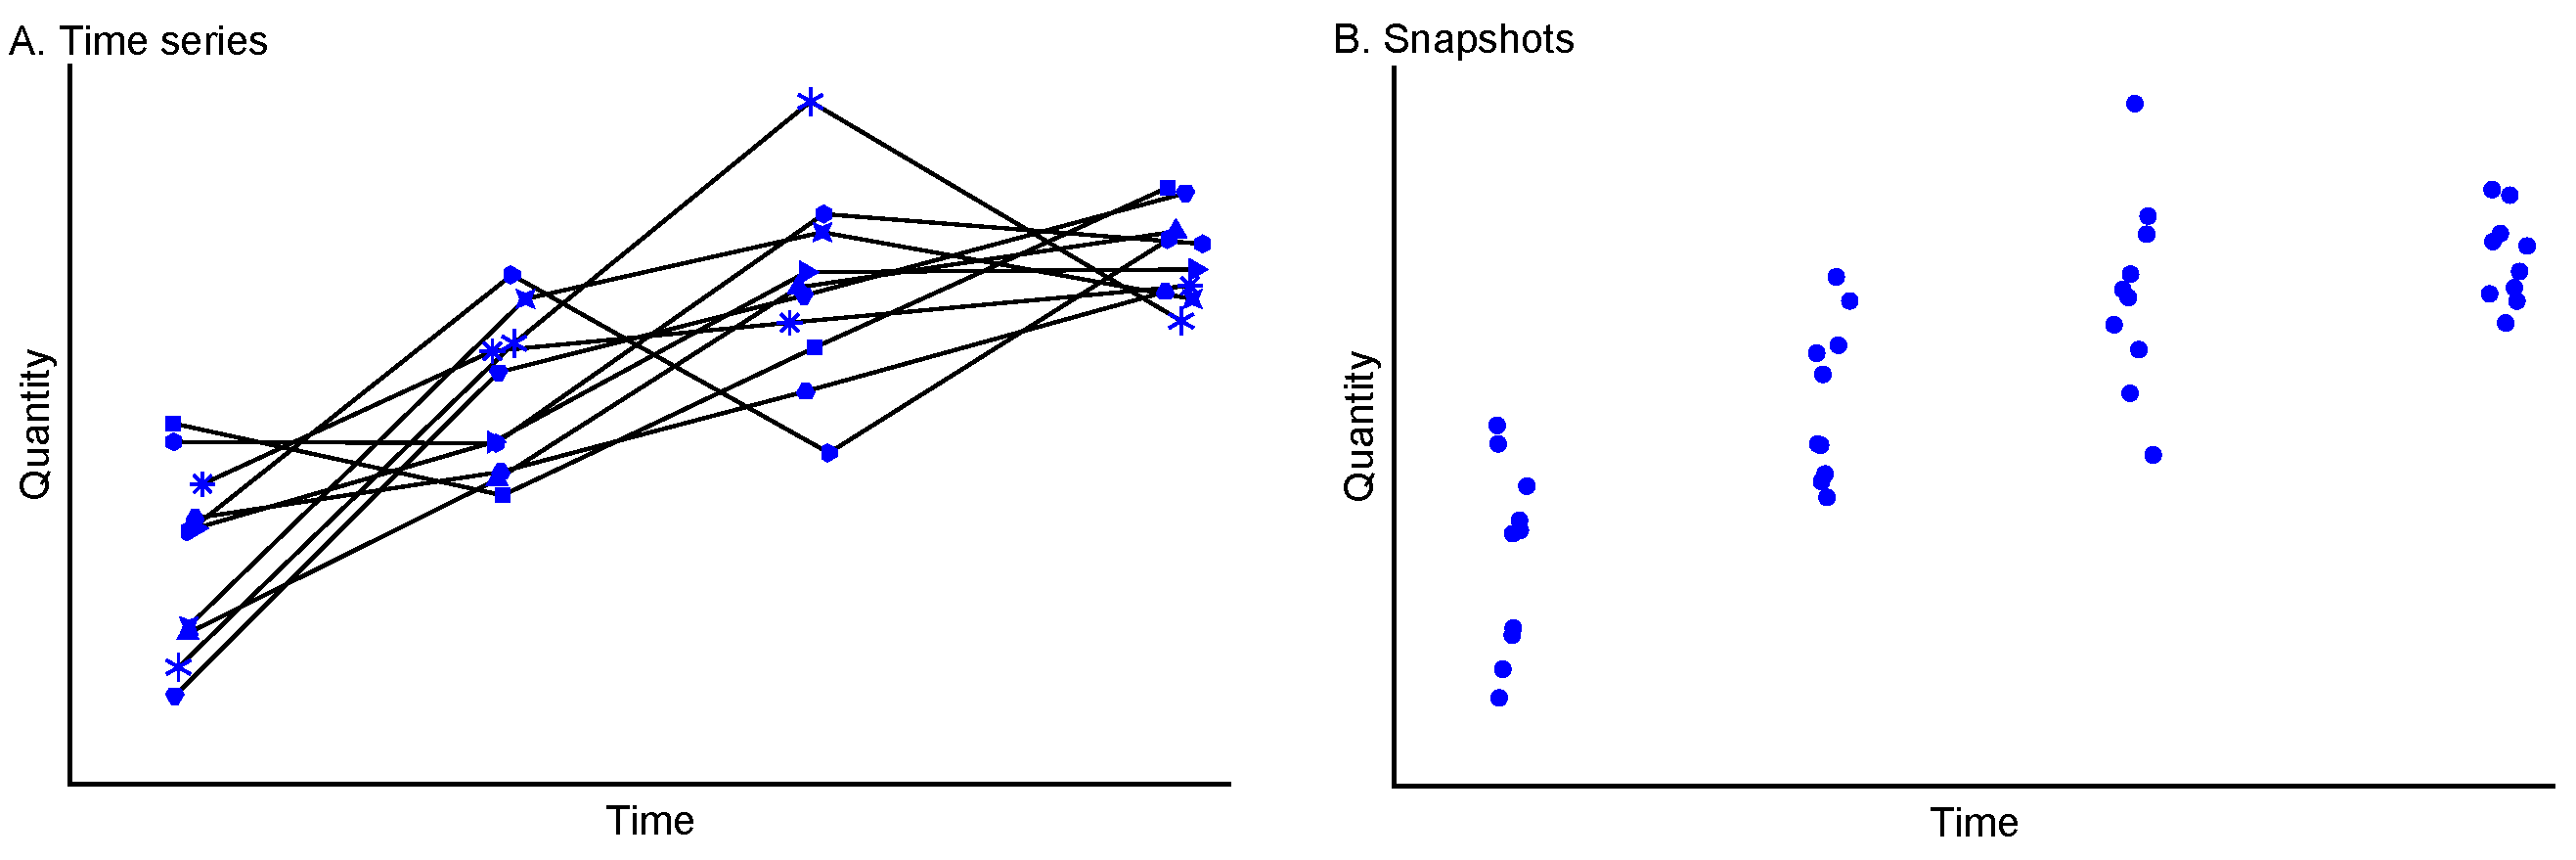
\includegraphics[width=\textwidth]{../figures/time_series_v_snapshots.pdf}}
	\caption{\textbf{Time series data (A) versus snapshot data (B) typical of single cell experiments.} In A that the cell identities are retained at each measurement point (indicated by given plot markers) whereas in the snapshot data in B, either this information is lost or, more often, cells are destroyed by the measurement process and so each observation corresponds to a distinct cell.}
	\label{fig:time_series_v_snapshots}
\end{figure}

We model the processes of an individual cell using a system of ordinary differential equations (ODEs), %where each element of the system describes the governing dynamics of a particular quantity of interest (for example, protein levels, RNA concentrations and so on),
%
\begin{equation}\label{eq:ode}
\begin{aligned}
\frac{d\boldsymbol{x}}{dt} &= \boldsymbol{f}(\boldsymbol{x}(t); \, \boldsymbol{\theta}), \quad \boldsymbol{f}: \R^k \times \R^p \mapsto \R^k, \\
\boldsymbol{x}(0) &= \boldsymbol{x}_0.
\end{aligned}
\end{equation}
%
Note that in most circumstances, the initial state of the system, $\boldsymbol{x}(0)$, is unknown and it is convenient to include these as elements of $\boldsymbol{\theta}$ to be estimated. %The solution of eq. (\ref{eq:ODE}) is given by $\boldsymbol{x}(t) = g(t; \boldsymbol{\theta})$, where $\boldsymbol{x}(t)\in\mathbb{R}^k$ is a vector of outputs at time $t$ and $g(.)$ is a function that typically won't be analytically-determined; instead approximated via a numerical integration scheme.


\subsection{Snapshot data}

In this paper, we assume variation characterised by snapshot data arises due to between-cell heterogeneity in the underlying parameters $\boldsymbol{\theta}$. Therefore, the evolution of the underlying state of cell $i$ is described by an idiosyncratic ODE,
%
\begin{equation} \label{eq:ode_i}
\begin{aligned}
\frac{d\boldsymbol{x}^{\{i\}}}{dt} &= \boldsymbol{f} \left( \boldsymbol{x}^{\{i\}}(t); \, \boldsymbol{\theta}^{\{i\}} \right),
                                      \quad \boldsymbol{f}: \R^k \times \R^p \mapsto \R^k, \\
\boldsymbol{x}^{\{i\}}(0) &= \boldsymbol{x}_0
\end{aligned}
\end{equation}
where $^{\{i\}}$ indicates the $i$th sample.
%
%with solution $\boldsymbol{x}^i(t) = g(t; \boldsymbol{\theta}^i)$.
The traditional (non-hierarchical) state-space approach to modelling dynamic systems supposes that measurement randomness generates output variation (Figure \ref{fig:data_generation}A). Our approach, by contrast, relies on the assumption that stochasticity in outputs is solely the result of variability in parameter values between cells (Figure \ref{fig:data_generation}B). Whether the assumption of ``perfect'' measurements is reasonable depends on the experimental details of  the system under investigation but we argue that our method nevertheless provides a useful approximation in many cases where the signal to noise ratio is high.

\begin{figure}[H]
	\centerline{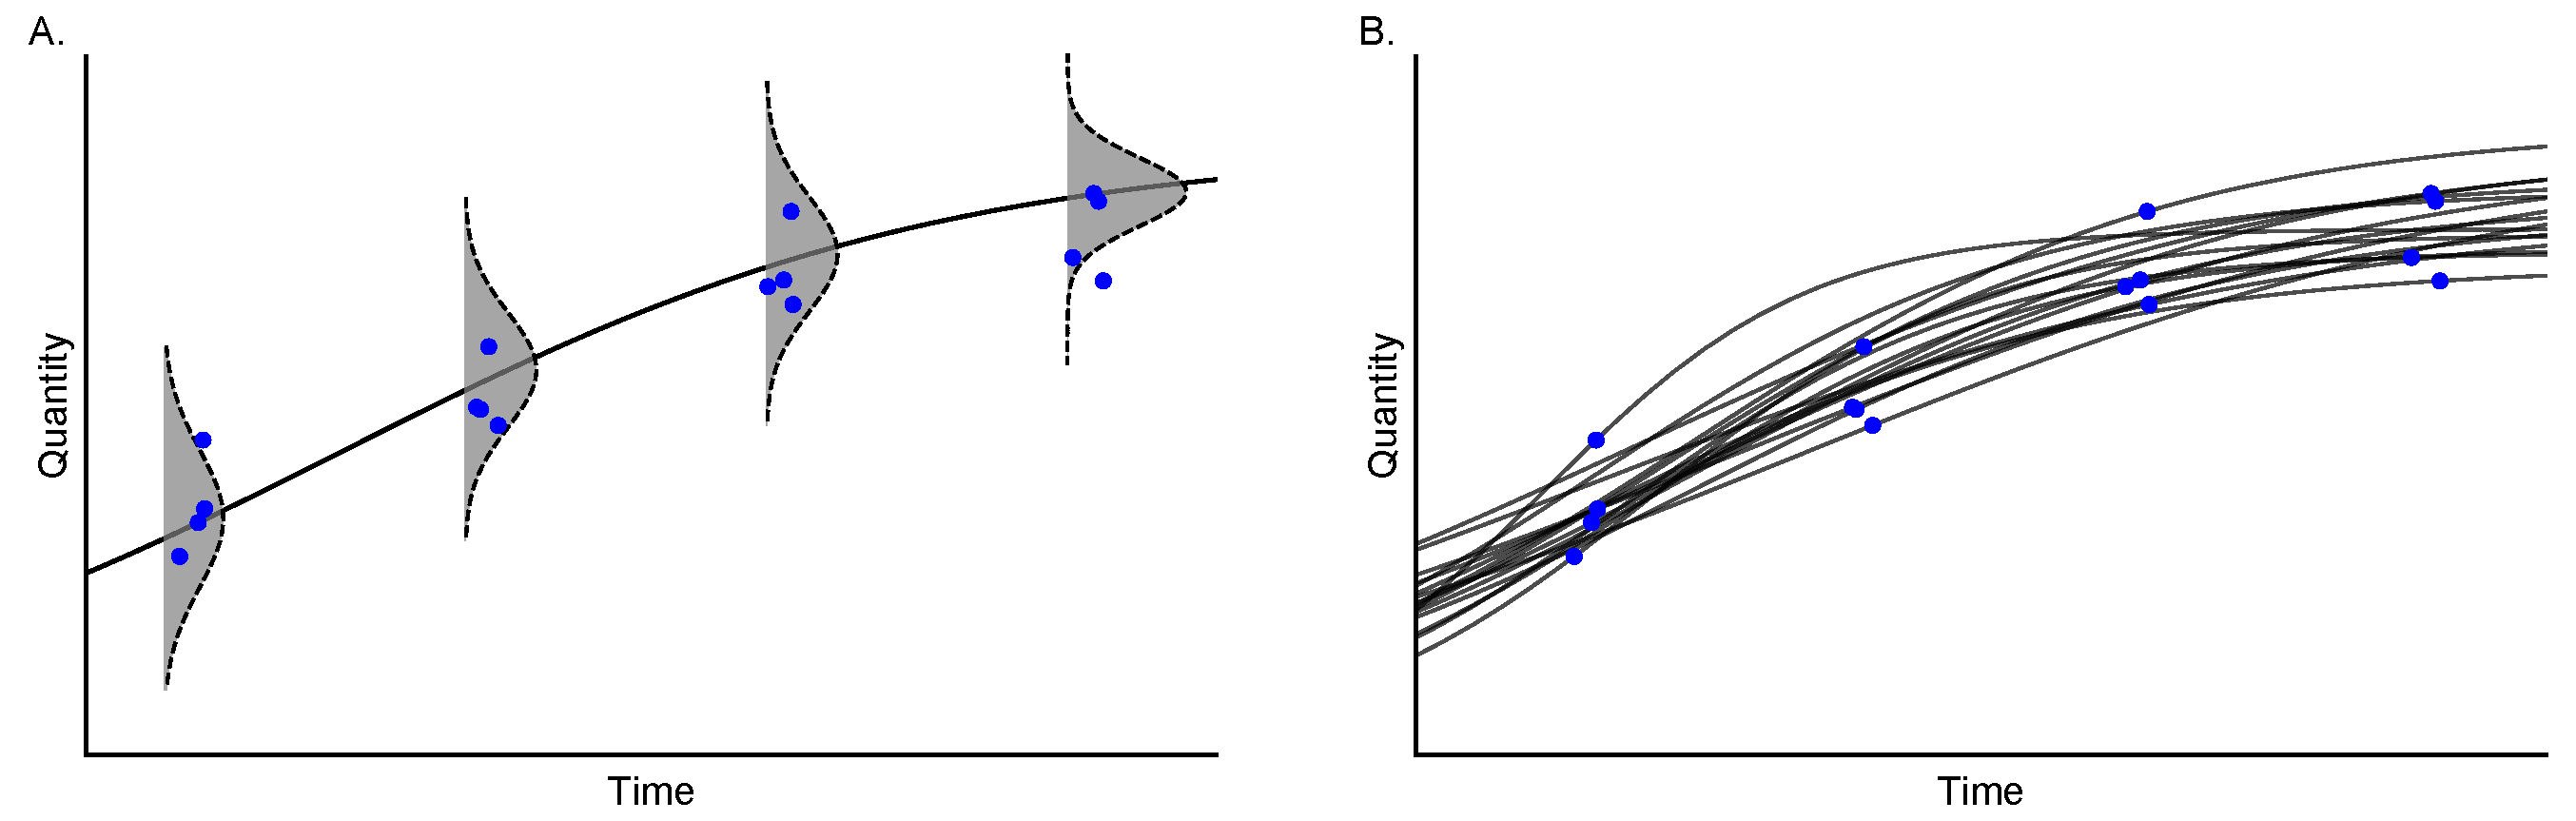
\includegraphics[width=\textwidth]{../figures/data_generation.pdf}}
	\caption{\textbf{Two ways to generate randomness in measured outputs: the state-space model (A) versus the parameter heterogeneity model (B).} For non-hierarchical state-space models (A), there is assumed to be a single ``true'' latent state where observations result from a noisy measurement process (grey histograms). For models with parameter heterogeneity (B), the uncertainty is generated by differences in cellular processes (black lines) between cells. Note that in both cases, individual cells are measured only once in their lifetime.}
	\label{fig:data_generation}
\end{figure}

\subsection{Emulation and representation of snapshot data}

We consider the situation in which we measure $m$ quantities of interest $q_j, j=1, \dots, m$.

We wish to emulate the experimental situation in which a set of observations is made. We simulate these experimental observations by solving the system of odes \eqref{eq:ode} multiple times for a range of values of parameters and calculate a (scalar-valued) quantity of interest for each value of the parameters.  Let $p(\boldsymbol{\theta})$ be a probability distribution characterising heterogeneity in cellular processes and consider the situation where we have $n_j$ observations of each quantity of interest $q_j$. These quantities of interest may be different functionals of the solution at the same time or the same functional at different times or a mixture of both. Define the vector containing a set of $m$ observations as
\begin{equation}
\boldsymbol{q}^\top = \left( q_1, q_2, \dots, q_m \right)
\end{equation}

\begin{algorithm}[H]
\label{alg:simulate}
\footnotesize
\texttt{\\}
\begin{algorithmic}
	\For{ $j=1$ to $m$ }
        \For{ $k=1$ to $n_j$ }
            \State $i=\sum_{l=1}^{j-1} n_l + k$
            \State Select $\boldsymbol{\theta}^{\{i\}} \sim p(\boldsymbol{\theta})$ and solve \eqref{eq:ode} for $\boldsymbol{x}^{\{i\}}(t)$.
            \State Compute $q_j\left( \boldsymbol{x}^{\{i\}}(t_j); \ \theta^{\{i\}} \right) \in \R$
        \EndFor
\EndFor
\end{algorithmic}
\caption{Emulation of experimental ``snapshot'' data}
\end{algorithm}
We define
\begin{equation}
\boldsymbol{y}(t_j)^\top = \left( q_j(\tilde x^{\{1\}}(t_j)), q_j(\tilde x^{\{2\}}(t_j)), \dots, q_j(\tilde x^{\{n_j\}}(t_j))  \right)^\top  \in \R^{n_j}
\end{equation}
and
\begin{equation}
  \boldsymbol{X}^\top = \left( \boldsymbol{y}(t_1), \boldsymbol{y}(t_2), \dots, \boldsymbol{y}(t_m) \right)^\top \in \R^s,
                        \quad \hbox{where} \; s = \sum_{j=1}^m n_j.
\end{equation}
The vector $\boldsymbol{X}$ defines the set of experimental observations, aka, raw snapshot data.

Raw snapshot data thus consists of measurements of individual cells with exact inference requiring simulating the underlying ODE system for each individual cell for each quantity of interest. This is cumbersome and impractical for the numbers of cells sampled in typical experimental setups and so, instead, we follow previous work and represent snapshot data using probability distributions \cite{hasenauer2011identification,hasenauer2014ode,loos2018hierarchical,dixit2018maximum}.
%The snapshots themselves can either be distributions of a single species or multiple species, which can be approximated by univariate and multivariate probability distributions respectively.
These probability distributions are characterised by parameter estimates $\hat{\Phi}$ for the output vector $\boldsymbol{Q}$ as determined by the output observations $\boldsymbol{X}$.
%The dimensionality of these probability distributions depends on the set of $m$ distinct observables $\tilde{\boldsymbol{x}}(\tilde{\boldsymbol{t}})=(x_{j_1}(t_1), x_{j_2}(t_2), ..., x_{j_m}(t_m))$ recorded by experimental measurements. Note that, $\tilde{\boldsymbol{x}}(\tilde{\boldsymbol{t}})$ corresponds to a particular set of measurements from a hypothetical cell and is distinct from $\boldsymbol{X}(\boldsymbol{t})$, which represents the full set of experimental outputs. The vector $\tilde{\boldsymbol{x}}(\tilde{\boldsymbol{t}})$ is hypothetical because in reality each cell is measured at a single timepoint (although we suppose measurements of different cellular attributes are possible contemporaneously).

The goal of our inference process is to  characterise the probability distribution $p(\boldsymbol{\theta}|\boldsymbol{X})$ representing heterogeneity in cellular processes. The first step in our inference workflow is to fit the output distributions using probability distributions (Figure \ref{fig:workflow}(i)). We assume that the volume of observational data means the estimated probability distributions are approximate sufficient statistics of the outputs, meaning $p(\boldsymbol{\theta}|\hat{\Phi}) \approx p(\boldsymbol{\theta}|\boldsymbol{X})$.

\begin{figure}[H]
	\centerline{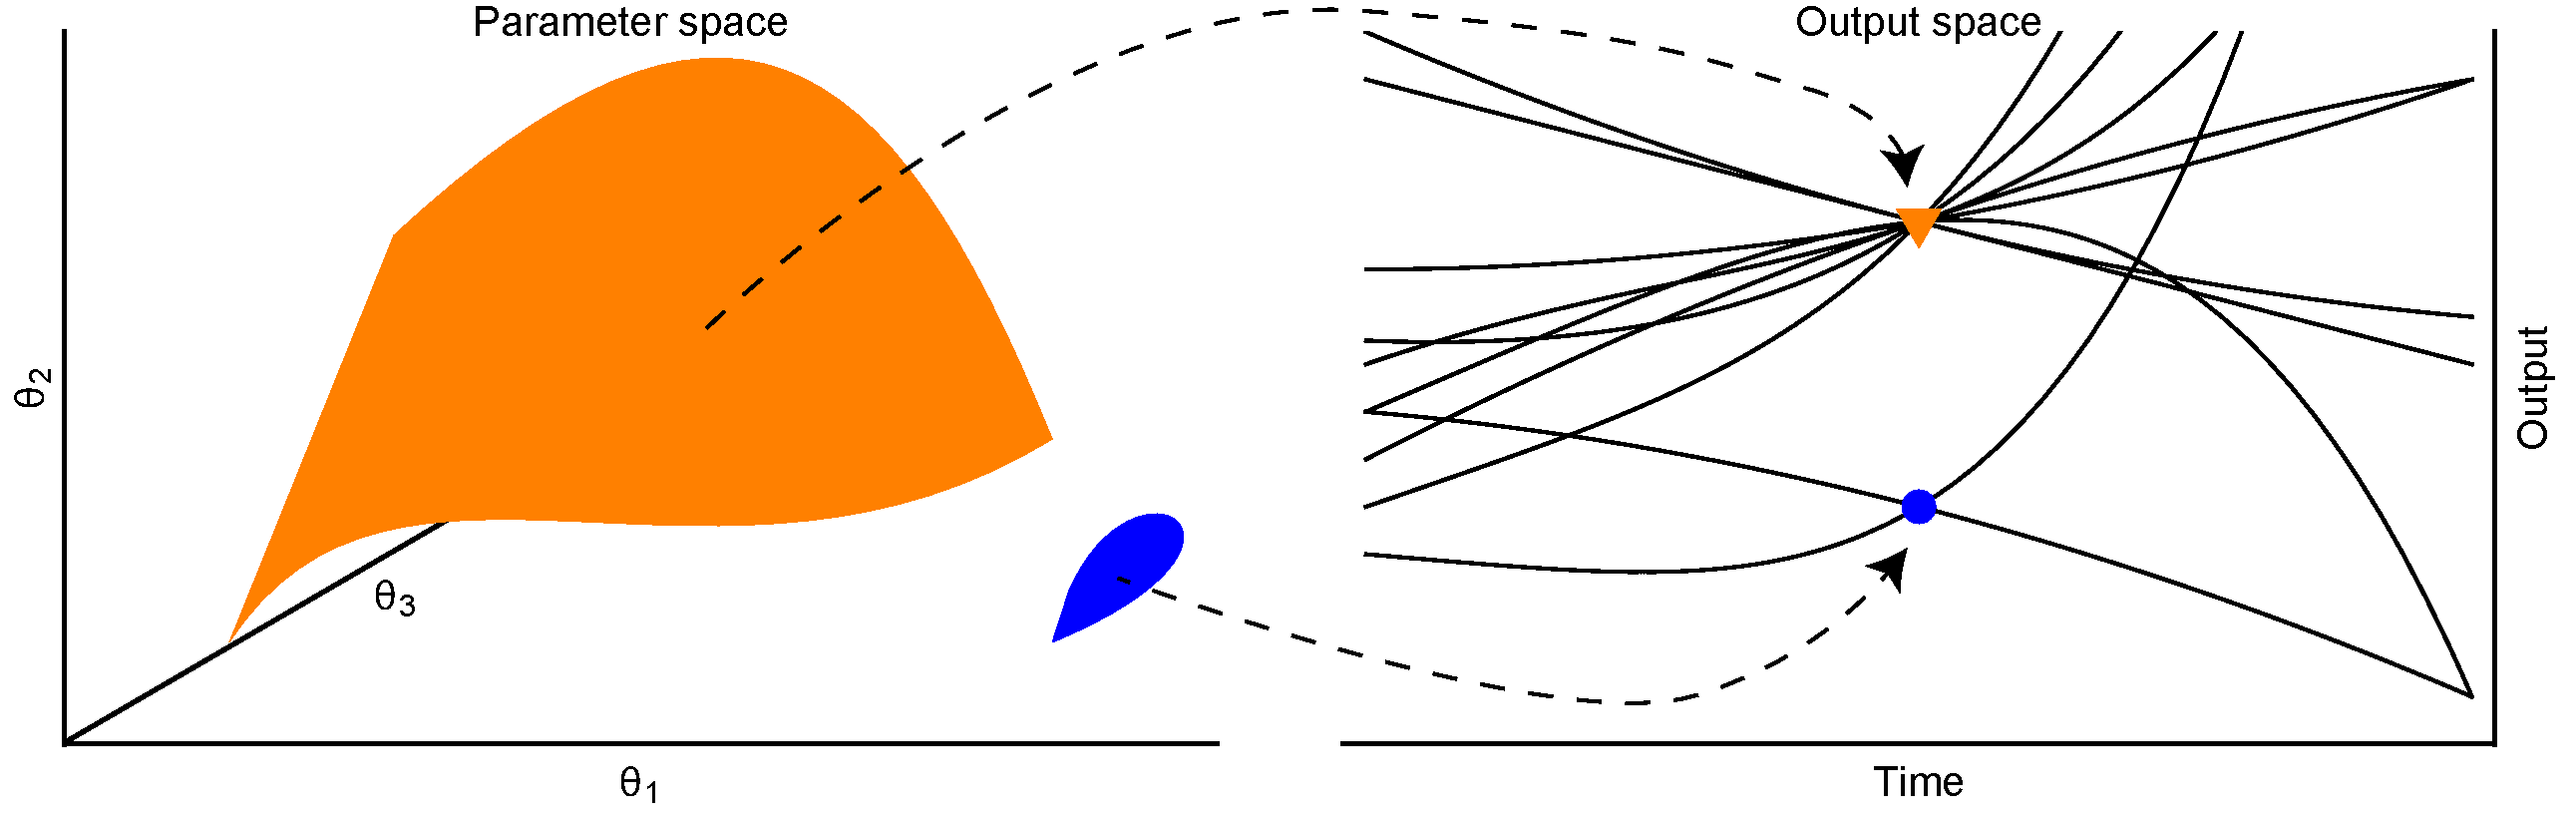
\includegraphics[width=\textwidth]{../figures/contour_volumes.pdf}}
	\caption{\textbf{The non-linear mapping from parameter values (left panel) to outputs (black lines; right panel) means different sized regions of parameter space (orange and blue surfaces; left panel) correspond to distinct output values (orange triangle and blue square; right panel).} In the right panel, each black line represents a distinct model simulation $g(t; \theta_1, \theta_2, \theta_3)$ and the triangle and square indicate outputs at a given point in time.}
	\label{fig:contour_volumes}
\end{figure}

\subsection{Notation}

\begin{table}[htbp]
\centering
%\scriptsize
\begin{adjustwidth}{0in}{0in}%
\begin{tabularx}{1.1\textwidth}{lll}
Variable	                                                & Definition                                   & Dimension \\
\toprule
$\boldsymbol{x}(t)$                                     	& ODE solution                                 & $\R^k$ \\
$\boldsymbol{\theta}$                                     	& ODE parameters                               & $\R^p$ \\
$\boldsymbol{f}(\boldsymbol{x}(t); \, \boldsymbol{\theta})$	& ODE RHS                                      & $\R^k$ \\
$\boldsymbol{x}^{\{i\}}(t)$                                 & ODE solution for cell $i$                    & $\R^k$ \\
&&\\
$q_j= q_j(\boldsymbol{x}(t_j))$                             & quantity of interest (qoi) $j$               & $\R^1$ \\
$\boldsymbol{q}= \left( q_1, \dots, q_m \right)$            & $m$ distinct qois                            & $\R^m$ \\
&&\\
$q_j^{\{i\}}= q_j(\boldsymbol{x}^{\{i\}}(t_j))$             & qoi $j$ for cell $i$                         & $\R^1$ \\
$\boldsymbol{y}_j=\left( q_j^{\{1\}}, \dots q_j^{\{n_j\}} \right)$  & qoi $j$ for cells $1, \dots, n_j$    & $\R^{n_j}$ \\
$\boldsymbol{X}=(\boldsymbol{y}_1,...,\boldsymbol{y}_m)$    & ``snapshot'' of all qoi                      & $\R^{\sum_{j=1}^m n_j}$ \\
&&\\
$\Phi$ & output target distribution $p(\boldsymbol{q}|\Phi)$              & $\R^m$ \\
$\Xi$  & prior parameter distribution $p(\boldsymbol{\theta}|\Xi)$        & $\R^p$ \\
$\Psi$ & prior output distribution $p(\boldsymbol{q}|\Psi)$               & $\R^p$ \\
&&\\
$\hat{a}$ & estimates of any quantity $a$                                                                  & - \\
&&\\
$\Omega(\boldsymbol{z})$              & parameter space mapping to $\boldsymbol{q}=\boldsymbol{z}$         & $\R^p$ \\
$\mathcal{V}(\boldsymbol{z})$         & volume of $\Omega(\boldsymbol{z})$                                 & $\R^+$ \\
$V$                                   & volume of parameter space                                          & $\R^+$ \\
\end{tabularx}
\caption{\textbf{Glossary of variable names used in this paper.}} %The dimensions of $\Phi$, $\Psi$ and $\Xi$ are listed as ``-'' since they depend on the form of the density used to represent the process and can be anywhere from $\mathbb{R}^1$ to $\mathbb{R}^\infty$. The variables are listed in the approximate order in which they appear in the text.}
\label{tab:variable_glossary}
\end{adjustwidth}
\end{table}




\subsection{Theoretical development of CMC}

We consider the underdetermined case where $m<p$, so that each of the quantities of interest can be generated from a set of parameter values and any
target output distribution $p(\tilde{\boldsymbol{q}}|\hat{\Phi})$ does not correspond to a unique parameter distribution.

%The models we seek to fit to snapshot data mostly cannot be identified from the observations. This is often because the number of model parameters exceeds the dimensionality of the output distribution (that is, $m>k$) meaning there typically exist non-singular sets of parameter values mapping to a single set of output values. That is, each vector of observed outputs $\tilde{\boldsymbol{q}}\in\mathbb{R}^m$, can often be caused by many combinations of parameters although, due to the non-linearity of the map from parameters to outputs, the ``volume'' of these regions of parameter space, $\mathcal{V}(\tilde{\boldsymbol{x}})$, is a function of output (Figure \ref{fig:contour_volumes}). In what follows, we make clear the distinction between observables $\tilde{\boldsymbol{x}}(\tilde{\boldsymbol{t}})$ and the vector-valued function representing modelled outputs $\boldsymbol{g}(\tilde{\boldsymbol{t}}; \boldsymbol{\theta})=(g_{j_1}(t_1; \boldsymbol{\theta}),g_{j_2}(t_2; \boldsymbol{\theta}),...,g_{j_m}(t_m; \boldsymbol{\theta}))\in\mathbb{R}^m$ since the latter is a function whereas that latter is a numeric value; we also drop the $\tilde{\boldsymbol{t}}$ notation from following expressions to minimise clutter.

%A consequence of this non-linear parameter to output geometry is that any target output distribution $p(\tilde{\boldsymbol{q}}|\hat{\Phi})$ does not correspond to a unique parameter distribution. For example, suppose $g(\theta_1, \theta_2) = \theta_1 + \theta_2$: the target distribution $\tilde{\boldsymbol{x}}\sim \mathcal{N}(0, 1)$ can be generated by any member of the set of parameter distributions $\sqrt{\eta} \theta_1 + \sqrt{1 - \eta} \theta_2$, where $\eta\in [0, 1]$ and $\theta_1, \theta_2 \sim \mathcal{N}(0, 1)$.

This means that in order to ensure uniqueness of the ``posterior'' parameter distributions, we are required to specify ``prior'' distributions for the parameters, as in more traditional Bayesian inference. An additional consequence of the degeneracy of the mapping from parameters to outputs is that any sampling algorithm aimed at exploring posterior parameter space must account for the differential volumes of iso-output contours. Whilst we refer the interested reader to our companion paper on this subject [citation for tutorial paper published in Open Science], we provide a quick derivation of the posterior parameter distribution which accounts for the non-linear mapping.

To derive the posterior distribution of parameter values $p(\boldsymbol{\theta}|\hat{\Phi})$, we consider the joint density of parameters and outputs $p(\boldsymbol{\theta},(\boldsymbol{q}|\hat{\Phi}))$. This can be decomposed in two ways,
%
\begin{equation}\label{eq:joint}
  p( \boldsymbol{\theta}, (\boldsymbol{q}|\hat{\Phi}) )
= p( \boldsymbol{\theta}|(\boldsymbol{q}, \hat{\Phi}) ) \times p(\boldsymbol{q}|\hat{\Phi})
= p( \boldsymbol{q}|(\boldsymbol{\theta}, \hat{\Phi}) ) \times p(\boldsymbol{\theta}|\hat{\Phi}).
\end{equation}
%
Rearranging to obtain the posterior parameter distribution,
%
\begin{equation}
p(\boldsymbol{\theta}|\hat{\Phi})
= \frac{p(\boldsymbol{\theta}|\boldsymbol{q}, \hat{\Phi}) \times p(\boldsymbol{q}|\hat{\Phi})}{p(\boldsymbol{q}| \boldsymbol{\theta}, \hat{\Phi})}.
\end{equation}
%
Given parameters $\boldsymbol{\theta}$, the mapping from parameters to outputs is deterministic meaning
$p(\boldsymbol{q}| \boldsymbol{\theta}, \hat{\Phi})=\delta(\boldsymbol{q}(\boldsymbol{\theta}),\boldsymbol{\theta})$ is the Dirac delta function centred at $\boldsymbol{q}=\boldsymbol{q}(\boldsymbol{\theta})$.


In what follows, we assume that the conditional distribution $p(\boldsymbol{\theta}|\boldsymbol{q}, \hat{\Phi})$ is independent of the data, meaning it represents a conditional ``prior'', which can be manipulated by Bayes' rule,
%
\begin{equation}\label{eq:prior}
p(\boldsymbol{\theta}|\boldsymbol{q}(\boldsymbol{\theta})) = \frac{p(\boldsymbol{\theta})}{p(\boldsymbol{q}(\boldsymbol{\theta}))},
\end{equation}
%
where we have used the Dirac delta function for $p(\boldsymbol{q}|\boldsymbol{\theta})$. This results in the form of the posterior parameter distribution targeted by our sampling algorithm,
%
\begin{equation}\label{eq:posterior_input}
p(\boldsymbol{\theta}|\hat{\Phi}) = \frac{p(\boldsymbol{\theta})}{p(\boldsymbol{q}(\boldsymbol{\theta}))} p(\boldsymbol{q}(\boldsymbol{\theta})|\hat{\Phi}).
\end{equation}
%
Again, we refer to our companion piece [citation] for detailed explanation of eqs. (\ref{eq:prior}) \& (\ref{eq:posterior_input}) and instead here provide brief interpretation when considering a uniform prior on parameter space. In this case, $p(\boldsymbol{\theta}) = \frac{1}{V}$, where $V$ is the total volume of parameter space. The denominator term of eq. (\ref{eq:prior}) is the prior induced on output space by the prior over parameter space. For a uniform prior on parameter values, this is %just proportion of parameter space where $\boldsymbol{g}(\boldsymbol{\theta}) = \tilde{\boldsymbol{x}}$, meaning,
%
\begin{equation}\label{eq:contour_volume}
p(\boldsymbol{\theta}|\boldsymbol{q}(\boldsymbol{\theta})) = \frac{1}{\mathcal{V}(\boldsymbol{q}(\boldsymbol{\theta}))},
\end{equation}
%
where $\mathcal{V}(\boldsymbol{q}(\boldsymbol{\theta}))$ is the volume of parameter space occupied by the iso-output region $\Omega(\tilde{\boldsymbol{q}}) = \{\boldsymbol{\theta}: \boldsymbol{q}(\boldsymbol{\theta}) = \tilde{\boldsymbol{q}}\}$. Therefore a uniform prior over parameter space implies a prior structure where all  parameter values resulting in the same output $\tilde{\boldsymbol{q}}$ are given equal weighting.

\subsection{Implementation of CMC}

\subsubsection{I. Estimation of $p(\boldsymbol{q}(\boldsymbol{\theta})$}

Except for some toy examples, the denominator of eq. (\ref{eq:prior}) cannot be calculated, and exact sampling from the posterior parameter distribution of eq. (\ref{eq:posterior_input}) is not, in general, possible. We propose instead a computationally efficient sampling method to estimate $p(\boldsymbol{q}(\boldsymbol{\theta}))$, which forms the first step of our so-called ``Contour Monte Carlo'' (CMC) algorithm (Algorithm \ref{alg:cmc}; Figure \ref{fig:workflow}(ii)), where we estimate the volume of iso-output contours with output value $\boldsymbol{q}(\boldsymbol{\theta})$. This step involves repeated independent sampling from the prior distribution of parameters $\boldsymbol{\theta}^{\{i\}}\sim p(\boldsymbol{\theta}|\Xi)$, where, for completeness, we have conditioned on $\Xi$ parameterising our probability density. Each parameter sample is then converted into an output value $\boldsymbol{q}^{\{i\}}=\boldsymbol{q}(\boldsymbol{\theta}^{\{i\}})$. The collection of output samples is then fitted using a vine copula kernel density estimator (KDE) \cite{nagler2016evading}, $(\boldsymbol{q}^{\{1\}},...,\boldsymbol{q}^{\{N_1\}})\sim p({\boldsymbol{q}}|\hat{\Psi})$. Throughout the course of development of CMC, we have tested many forms of KDE and have found vine copula KDE is best suited to approximating the higher dimensional probability distributions required in practice.


\subsubsection{Step II. MCMC sampling of posterior}

The second step in our algorithm then uses Markov chain Monte Carlo (MCMC) to sample from an approximate version of eq. (\ref{eq:posterior_input}) with the estimated density $p(\boldsymbol{q}(\boldsymbol{\theta})|\hat{\Psi})$ replacing its corresponding estimand (Algorithm \ref{alg:cmc}; Figure \ref{fig:workflow}(iii)),
%
\begin{equation}\label{eq:posterior_input_estimated}
p(\boldsymbol{\theta}|\hat{\Phi},\Xi,\hat{\Psi}) =
\frac{p(\boldsymbol{\theta}|\Xi)}{p(\boldsymbol{q}(\boldsymbol{\theta})|\hat{\Psi})} \,
p(\boldsymbol{q}(\boldsymbol{\theta})|\hat{\Phi}).
\end{equation}
%

\subsubsection{Step III. Reconstruction of target output distribution}

The final step in CMC is to compare output samples generated from the result of the MCMC calculation with the target distribution (Figure \ref{fig:workflow}(iv)). Asymptotically (in terms of the sample size of both sampling steps), CMC produces a sample of parameter values $(\boldsymbol{\theta}^{\{1\}},\boldsymbol{\theta}^{\{2\}},...)$ which, when mapped to the output space, corresponds to the target distribution $\hat{\Psi})$. In developing CMC, we have found that a finite sample of modest size for both steps of CMC results in parameter samples that, when transformed, often represent reasonable approximations of the target. There are however occasions when this is not the case and we have found this final confirmatory step indispensable since it frequently highlights inadequacies in the contour volume estimation or the MCMC, meaning more samples from either or both of these steps are required. It may also be necessary to tweak hyperparameters of the KDE to ensure reasonable approximation in the contour volume estimation step. If the target distribution is sensitive to the contour volume estimates, this may also indicate that the target snapshot distribution is incompatible with the model: here, we make no claims on existence of a solution to the inverse problem, only that, if one should exist, Contour Monte Carlo is a pragmatic approach to approximate it by sampling. A useful way to diagnose whether the target distribution can be produced from the model and specified priors is to examine the output values from the contour volume estimation step of CMC. If the majority of probability mass of the target lies outside the bounds of the bulk simulated output values obtained by independent sampling from the prior, then the model and/or chosen prior is unlikely to be invertible to this particular target.

\subsubsection{Workflow and CMC algorithm}

A graphical illustration of the complete CMC workflow is provided in Figure \ref{fig:workflow}. All variables are defined in Table \ref{tab:variable_glossary}.

\begin{figure}[H]
\label{fig:workflow}
\centerline{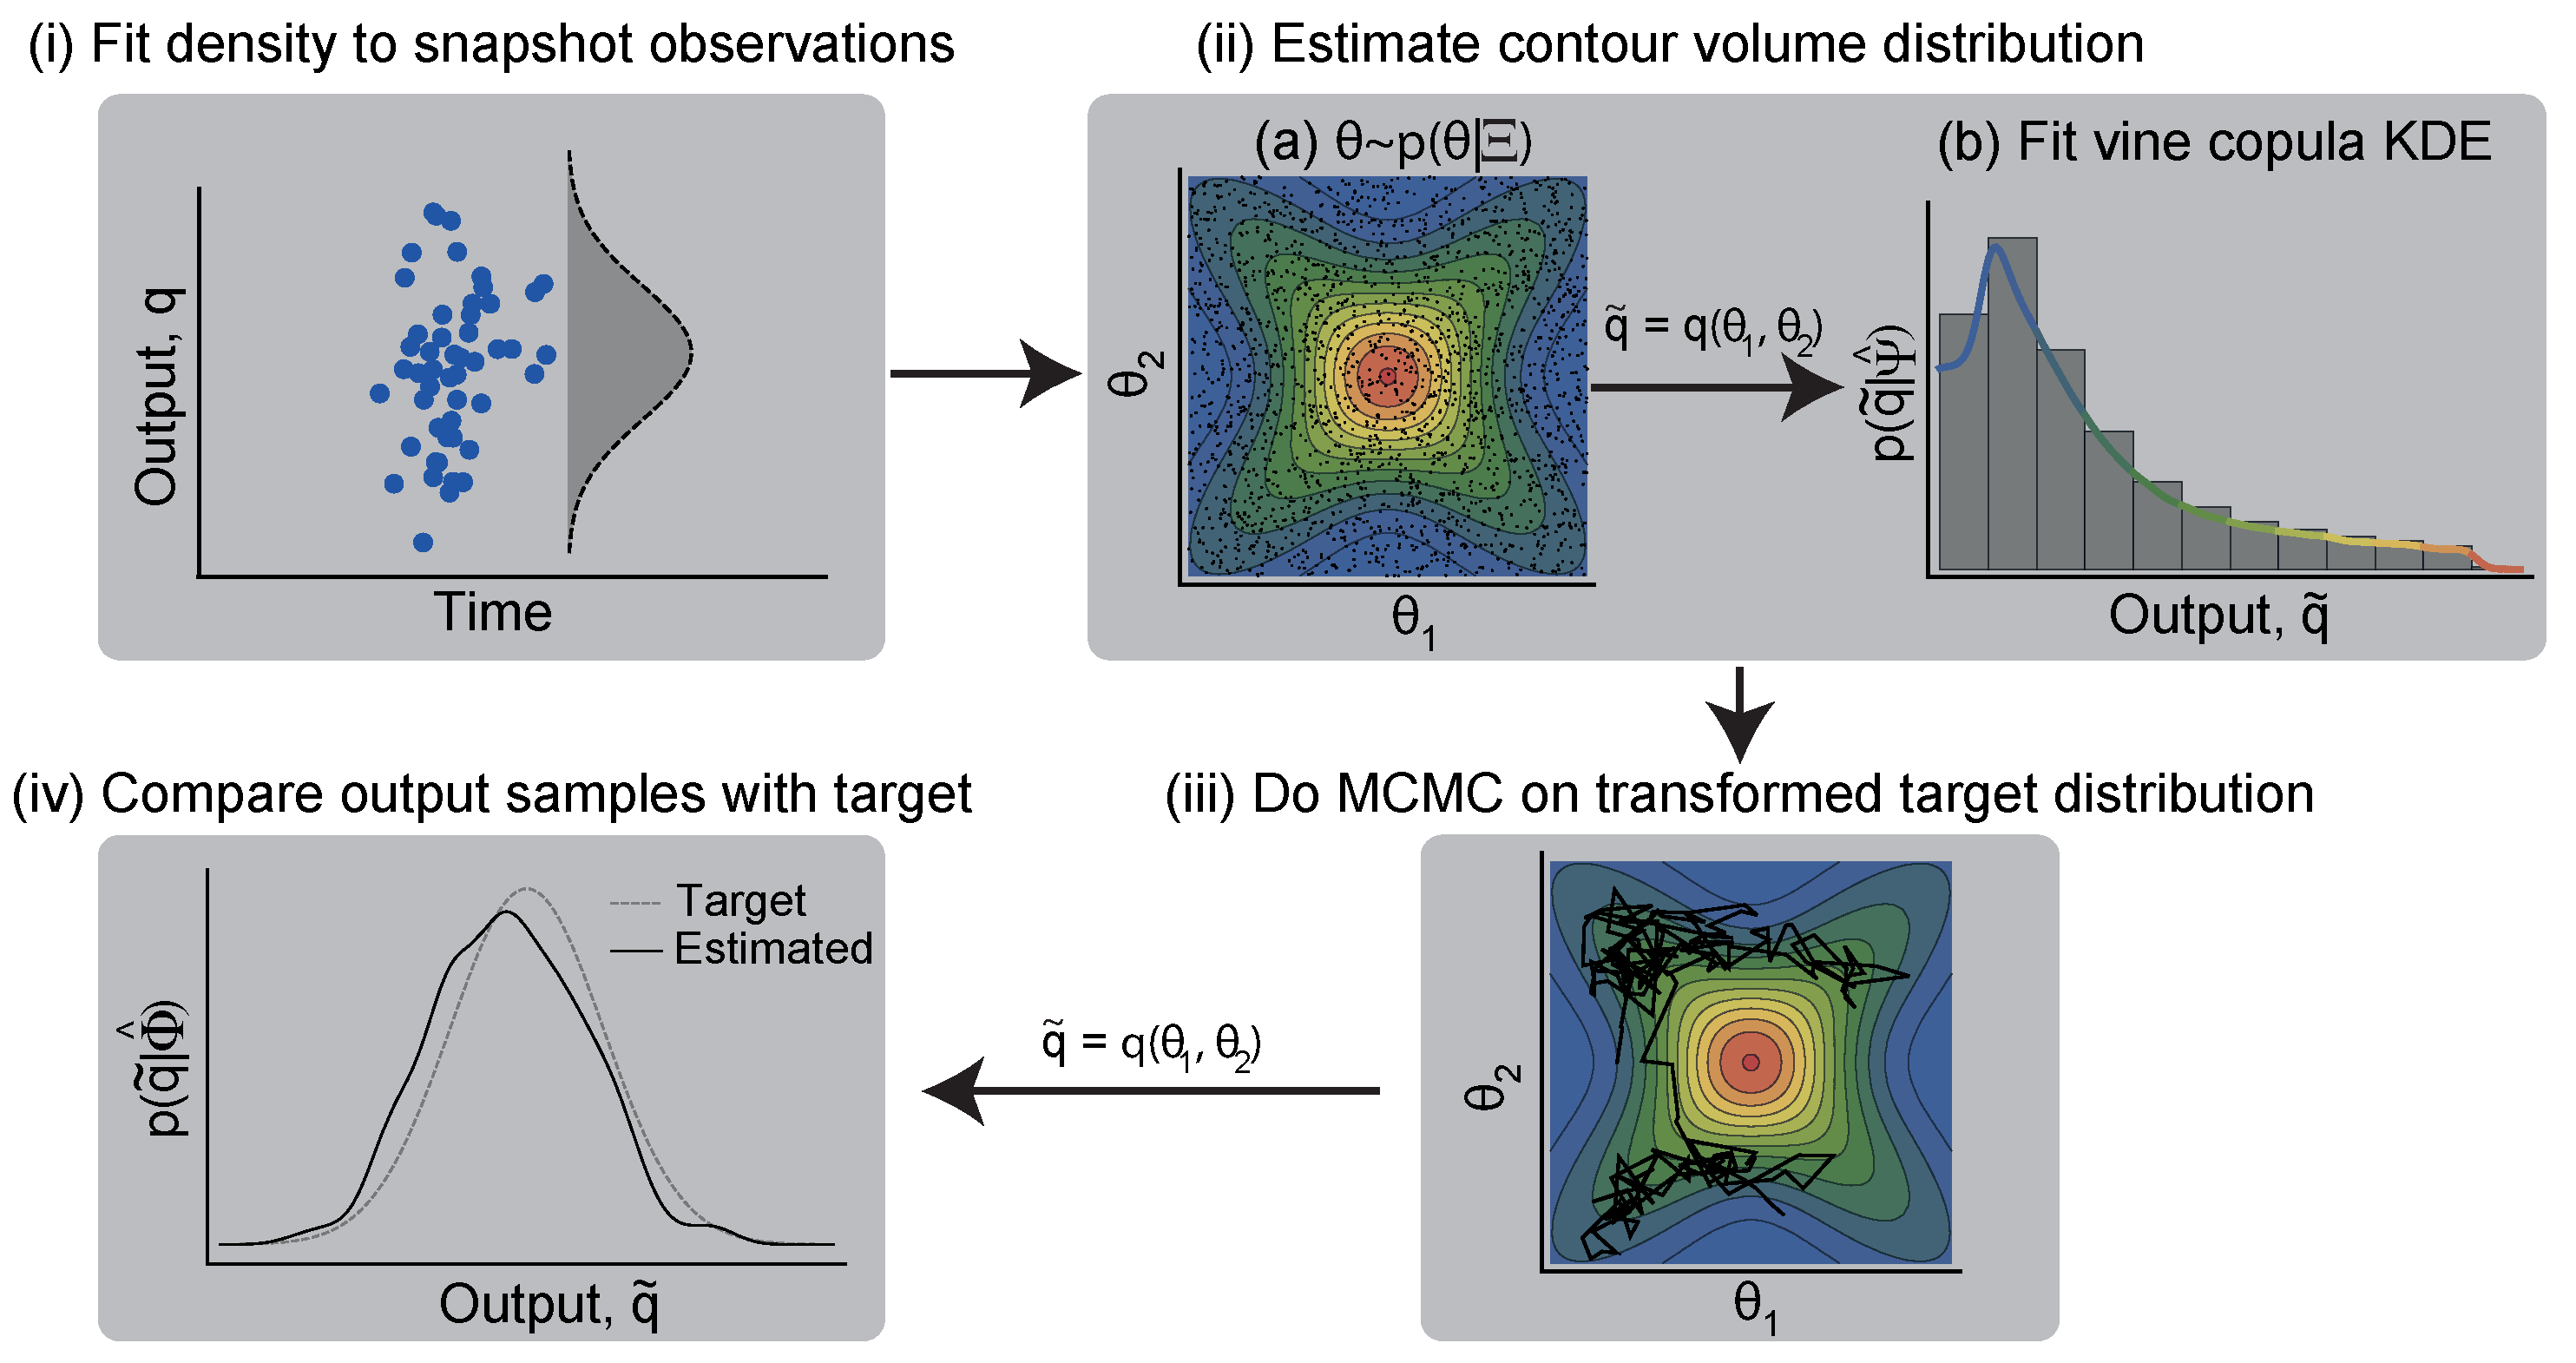
\includegraphics[width=\textwidth]{../figures/workflow.pdf}}
\caption{\textbf{The workflow for Contour Monte Carlo to estimate cell population heterogeneity.}
The distribution targeted in (iii) is given by eq. (\ref{eq:posterior_input_estimated}).}
\end{figure}

The CMC algorithm is provided in Algorithm \ref{alg:cmc}. A definition of all variables is provided in Table \ref{tab:variable_glossary}. For simplicity, in this implementation MCMC sampling is performed via the Random Walk Metropolis algorithm, but for the examples in \S \ref{sec:results}, we use an adaptive MCMC algorithm \cite{johnstone2016uncertainty}.

\begin{algorithm}[H]
\footnotesize
\texttt{\\}
\begin{algorithmic}
\Procedure{CMC}{$\boldsymbol{X}, \Xi, N_1, N_2$}\Comment{Sample from posterior parameter distribution}
	\State $\hat{\Phi} = \Call{SnapshotEstimator}{\boldsymbol{X}}$
	\State $\hat{\Psi} = \Call{ContourVolumeEstimator}{\Xi,N_1}$
	\State $\left(\boldsymbol{\theta}^{\{1\}},...,\boldsymbol{\theta}^{\{N_2\}}\right) = \Call{MCMC}{\hat{\Phi},\Xi, \hat{\Psi},N_2}$
	\State $\text{converged} = \Call{CompareOutputToTarget}{(\boldsymbol{\theta}_1,...,\boldsymbol{\theta}_{N_2}), \hat{\Phi}}$
	\If{converged$\neq$1} \Comment{Rerun contour volume estimation and/or MCMC}
		 \State $\Call{ContourVolumeEstimator}{\Xi, N_1'},\; N_1' > N_1$
         \State $\left( \boldsymbol{\theta}^{\{1\}},...,\boldsymbol{\theta}^{\{N_2'\}} \right)
                = \Call{MCMC}{\hat{\Phi},\Xi, \hat{\Psi},N_2'}, \; N_2' > N_2$
         \State $N_1 \leftarrow N_1', \; N_2 \leftarrow N_2'$
	\EndIf
	\State \Return $\left( \boldsymbol{\theta}^{\{1\}},...,\boldsymbol{\theta}^{\{N_2\}} \right)$
\EndProcedure
\end{algorithmic}

\texttt{\\}
\begin{algorithmic}
\Procedure{SnapshotEstimator}{$\boldsymbol{X}$}\Comment{Fit density to snapshot observations}
	\State $\boldsymbol{X} \sim p(\boldsymbol{q}|\hat{\Phi})$
	\State \Return $\hat{\Phi}$
\EndProcedure
\end{algorithmic}
	
\texttt{\\}
\begin{algorithmic}
\Procedure{ContourVolumeEstimator}{$\Xi, N_1$}\Comment{Estimate volume of contours}
	\For{$i$ in $1:N_1$}
		\State $\boldsymbol{\theta}^{\{i\}} \sim p(\boldsymbol{\theta}|\Xi)$           \Comment{Sample from prior density}
		\State $\boldsymbol{q}^{\{i\}} = \boldsymbol{q}(\boldsymbol{\theta}^{\{i\}})$  \Comment{Calculate corresponding output value}
	\EndFor
	\State $\left( \boldsymbol{q}^{\{1\}}, \dots ,\boldsymbol{q}^{\{N_1\}} \right) \sim p(\tilde{\boldsymbol{q}}|\hat{\Psi})$
           \Comment{Fit vine copula kernel density estimator}
	\State \Return $\hat{\Psi}$
\EndProcedure
\end{algorithmic}

\texttt{\\}
\begin{algorithmic}
\Procedure{MCMC}{$\hat{\Phi},\Xi, \hat{\Psi}, N_2$}\Comment{Random Walk Metropolis algorithm targeting posterior parameter distribution.}
	\State $\boldsymbol{\theta}^{\{0\}} \sim \pi(.)$ \Comment{Sample from arbitrary initialisation distribution}
	\For{$i$ in $1:N_2$}
		\State $\boldsymbol{\theta}^{\{i\}^\prime}\sim \mathcal{N}(\boldsymbol{\theta}^{\{i-1\}},\boldsymbol{\Sigma})$ \Comment{Propose new parameter values for parameters}
		\State $r = \left[
                     p(\boldsymbol{\theta}^{\{i^\prime\}}|\Xi) \
                     p(\boldsymbol{q}(\boldsymbol{\theta}^{\{i\}})|\hat{\Psi}) \
                     p(\boldsymbol{q}(\boldsymbol{\theta}^{\{i^\prime\}})|\hat{\Phi})\right]
                     /
                     \left[
                     p(\boldsymbol{\theta}^{\{i\}}|\Xi) \
                     p(\boldsymbol{q}(\boldsymbol{\theta}^{\{i^\prime\}})|\hat{\Psi}) \
                     p(\boldsymbol{q}(\boldsymbol{\theta})|\hat{\Phi})
                     \right]$\Comment{Metropolis acceptance ratio.}
		\State $u\sim U(0,1)$ \Comment{Sample from uniform distribution}
		\If{$r > u$}
		    \State $\boldsymbol{\theta}^{\{i\}} = \boldsymbol{\theta}^{\{i^\prime\}}$ \Comment{Accept proposal}
		\Else
		    \State $\boldsymbol{\theta}^{\{i\}} = \boldsymbol{\theta}^{\{i-1\}}$ \Comment{Reject proposal}
		\EndIf
	\EndFor
	\State \Return $\left( \boldsymbol{\theta}^{\{1\}},...,\boldsymbol{\theta}^{\{N_2\}} \right)$
\EndProcedure
\end{algorithmic}

\texttt{\\}
\begin{algorithmic}
\Procedure{CompareOutputToTarget}{$(\boldsymbol{\theta}_1,...,\boldsymbol{\theta}_{N_2}), \hat{\Phi}$}\Comment{Check output distribution close to target}
	\For{$i$ in $1:N_2$}
		\State $\tilde{\boldsymbol{q}}_i = \boldsymbol{q}(\boldsymbol{\theta}_i)$ \Comment{Compute output for each parameter sample}
	\EndFor
	\If{$\left( \tilde{\boldsymbol{q}}_1,\dots,\tilde{\boldsymbol{q}}_{N_2} \right)
              \sim p(\tilde{\boldsymbol{q}}|\hat{\Phi})?$} \Comment{Compare outputs with target}
		\State \Return 1 \Comment{If outputs sufficiently close then converged}
	\Else
		\State \Return 0
	\EndIf
\EndProcedure
\end{algorithmic}

\caption{Pseudocode for the Contour Monte Carlo algorithm for sampling from the posterior parameter distribution of eq. (\ref{eq:posterior_input_estimated}). }\label{alg:cmc}
\end{algorithm}


\subsection{Future refinements}
In generating our results in \S\ref{sec:results}, for the contour volume estimation step, we assumed sample sizes were sufficient if the output samples from the MCMC provided a reasonable approximation to the target, although we recognise that future work should refine this process further. For the MCMC step, we use adaptive covariance MCMC (see SOM of \cite{johnstone2016uncertainty}) to sample from the target distribution, as we have found that it provides a considerable speed-up over Random Walk Metropolis \cite{metropolis1953equation,lambert2018Student}. We also use the Gelman-Rubin convergence statistic $\hat{R}$ which provides a heuristic measurement of convergence \cite{lambert2018Student,gelman1992inference}, and use a threshold of $\hat{R}\leq\sim 1.1$ to diagnose convergence.

\section{Results}\label{sec:results}
In this section, we use CMC to estimate posterior parameter distributions for four biological systems. In two of the examples, we assume that the first step of CMC (``SnapshotEstimator'' within Algorithm \ref{alg:cmc}) has already been completed, and we are faced with inferring a parameter distribution which, when mapped to outputs, recapitulates the target density. To accompany the text, we provide the Julia notebook used to generate the results. A table of priors used for each example is provided in Table \ref{tab:priors}.


\subsection{Growth factor model}
We first consider the ``growth factor model'' introduced by \cite{dixit2018maximum}, which concerns the dynamics of inactive ligand-free cell surface receptors, $R$, and active ligand-bound cell surface receptors, $P$, modulated by an exogenous ligand, $L$. The governing dynamics are determined by the following system,
%
\begin{align}\label{eq:growth_factor}
\frac{dR}{dt} &= R_T k_{deg} + k_1 L R(t) + k_{-1} P(t) - k_{deg} R(t)\\
\label{eq:growth_factor1}
\frac{dP}{dt} &= k_1 L R(t) - k_{-1} P(t) - k^*_{deg} P(t),
\end{align}
with initial conditions,
\begin{equation*}
R(0) = 0.0, \qquad P(0) = 0.0,
\end{equation*}
%
and $\boldsymbol{\theta}=(R_T, k_1, k_{-1}, k_{deg}, k^*_{deg})$ are parameters to be determined. In this example, we use measurements of the active ligand-bound receptors $P$ to estimate cellular heterogeneity in these processes. We denote the solution of eq. (\ref{eq:growth_factor1}) as $P(t; \boldsymbol{\theta}, L)$. Here we generate a target model by forward simulations of eq. \eqref{eq:growth_factor}; in each case recording $(P(10; \boldsymbol{\theta}, 2), P(10; \boldsymbol{\theta}, 10))$. In each forward simulation, we fix $(k_{-1}, k_{deg}, k^*_{deg}) = (8, 0.015, 0.25)$ and independently sample values ${R_T\sim \mathcal{N}(6.5\times 10^5, 0.6\times 10^4)}$ and ${k_1\sim \mathcal{N}(1.7, 0.05)}$. This generates an output distribution approximately given by,
%
\begin{equation}\label{eq:MM_outputDistribution}
\boldsymbol{q} =
\begin{pmatrix}
q_1\\
q_2\\
\end{pmatrix}
=
\begin{pmatrix}
P(10; \boldsymbol{\theta}, 2)\\
P(10; \boldsymbol{\theta}, 10)\\
\end{pmatrix} \sim  \mathcal{N}
\begin{bmatrix}
\begin{pmatrix}
2\times 10^4\\
3\times 10^4\\
\end{pmatrix}, \;\;
\begin{pmatrix}
1\times 10^5 & 0\\
0 & 1\times 10^5\\
\end{pmatrix}
\end{bmatrix}.
\end{equation}
%
We note that, whilst the parameters $(k_{-1}, k_{deg}, k^*_{deg})$ are fixed during this step (to generate output distributions), they are allowed to vary in \S\ref{sec:growthmodel_uniform} and \S\ref{sec:growthmodel_gaussian} (where we use CMC to perform inference).

\subsubsection{Uniform prior}\label{sec:growthmodel_uniform}
For an under-determined model, the number of QOIs, $m$, is less than the number of parameters, $p$, and there typically exists a non-singular set of parameter distributions mapping to the same target output distribution. To uniquely identify a posterior parameter distribution, it is, therefore, necessary to specify a prior parameter distribution. By incorporating priors, this allows pre-existing biological knowledge to be included, leading to reduced uncertainty in parameter estimates. CMC allows any prior with correct support to be used. Changes to priors affect both the ``ContourVolumeEstimation'' and ``MCMC'' steps of CMC (Algorithm \ref{alg:cmc}), so that the (changed) posterior parameter distribution still maps to the target.

To start, we specify a uniform prior for each of the five parameters, with bounds given in Table \ref{tab:priors}, and use CMC to estimate the posterior parameter distribution. In Figure \ref{fig:growth_factor_outputs}A, we show the sampled outputs (blue points) versus the contours of the target distribution (black solid closed curves), illustrating a good correspondence between the sampled and target densities. Above and to the right of the main panel, we also display the marginal target densities (solid black lines) versus kernel density estimator reconstructions of the output marginals from the CMC samples (dashed blue lines), which again highlights the fidelity of the CMC sampled density to the target.

\begin{figure}[H]
	\centerline{\includegraphics[width=\textwidth]{../figures/growth_factor_outputs.pdf}}
	\caption{\textbf{Growth factor model. Target joint output distribution (solid contour lines) and target marginal distributions (solid lines; above and to the right of each figure) versus outputs sampled by CMC (blue points) and reconstructed marginals (dashed lines). (A) uniform priors. (B) Gaussian priors.} In CMC, 100,000 independent samples were used in the ``ContourVolumeEstimator'' step and 10,000 MCMC samples across each of 4 Markov chains were used in the second step, with the first half of the chains discarded as ``warm-up'' \cite{lambert2018Student}. For the reconstructed marginal densities in the plots, we use Mathematica's ``SmoothKernelDistribution'' function specifying bandwidths of 100 with Gaussian kernels \cite{mathematica}.}
	\label{fig:growth_factor_outputs}
\end{figure}


In Figure \ref{fig:growth_factor_inputs}A, we plot the joint posterior parameter distribution for $k_1$, the rate of ligand binding to inactive receptors and $k_{-1}$, which dictates the rate of the reverse reaction. A given level of bound ligands can be generated in many different ways. Not surprisingly, it is the \emph{ratio} of the forward and reverse reaction rates, $k_1$ and $k_{-1}$ respectively, that is of greatest importance, and because of this, the distribution representing cell process heterogeneity contains linear positive correlations between these parameters.


In Figure \ref{fig:growth_factor_inputs}B, we show the posterior parameter distribution for $k_{deg}$, the rate of degradation of ligand-free cell surface receptors and $R_T$, the rate of introduction of ligand-free cell surface receptors. This plot shows more concentrated posterior mass than in Figure \ref{fig:growth_factor_inputs}A.


Why do our measurements allow us to better resolve $(k_{deg},R_T)$ compared to $(k_1,k_{-1})$? To answer this, it is useful to calculate the sensitivity of $P(t; \boldsymbol{\theta}, L)$ to changes in each of the parameters. To account for the differing magnitudes of each parameter, we calculate elasticities, the proportional changes in measured output for a proportional change in parameter values, using the forward sensitivities method described in \cite{DGCT2018}, and these are shown in Figure \ref{fig:dixit_elasticities}. When the exogenous ligand is set at $L=2$, these indicate the active ligand-bound receptor concentration is most elastic to changes in $R_T$ and $k_{deg}$. This higher elasticity means that their range is more restricted by the output measurement than for $k_1$ and $k_{-1}$, which have much smaller elasticities at $t=10$. In Table \ref{tab:growth_factor_results}, we show the posterior quantiles for the estimated parameters, and in the last column, indicate the ratio of the 25\%-75\% posterior interval widths to the uniform prior range for each parameter. These were strongly negatively correlated with the magnitude of the elasticities for each parameter ($\rho=0.95$, $t=-5.22$, $df=3$, $p=0.01$ for Pearson's product-moment correlation), indicating the utility of sensitivity analyses for optimal experimental design, see e.g., \cite{Banks2011}. We suggest, however, that CMC can also be used for this purpose. If an experimenter generates synthetic data for various choices of QOIs, they can use CMC to derive the posterior parameter distributions in each case. They then, simply, select the particular QOI producing the narrowest posterior for key parameters.

In both panels of Figure \ref{fig:growth_factor_inputs}, we also plot the ``\textit{actual}'' parameter values as dashed lines: for $k_{-1}$ and $k_{deg}$, these indicate the true (fixed) parameter values, and, for $k_1$ and $R_T$, they show the mean of each Gaussian sampling distribution ($\pm$ two standard deviations shown by shaded rectangles). For most parameters, these indicate that the area of highest posterior density is close to the causative parameter values. This is reaffirmed in the top panel of Table \ref{tab:growth_factor_results}, where, in all cases, the actual parameter values lie within the estimated 95\% quantiles for each parameter -- indicating that the parameters were reasonably well identified.


\begin{figure}[H]
	\centerline{\includegraphics[width=\textwidth]{../figures/growth_factor_inputs.pdf}}
	\caption{\textbf{Growth factor model. Joint posterior distributions estimated by CMC. Top row (A-B): $(k_1,k_{-1})$ and $(k_{deg},R_T)$ using uniform priors. Bottom row (C-D): $(k_1,k_{-1})$ and $(k_{deg},R_T)$ using Gaussian priors.} In all panels, dashed lines indicate the parameter set or distribution used to generate the target distribution given by eq. \eqref{eq:MM_outputDistribution}: for $k_{-1}$ and $k_{deg}$, the dashed lines show true parameter values and for $k_1$ and $R_T$, they show the mean of each Gaussian sampling distributions ($\pm$ two standard deviations shown by shaded rectangles). See Figure \ref{fig:growth_factor_outputs} caption for CMC details and Table \ref{tab:priors} for the priors used. Red (blue) indicates areas of relatively high (low) probability density.}
	\label{fig:growth_factor_inputs}
\end{figure}

\begin{figure}[H]
	\centerline{\includegraphics[width=0.7\textwidth]{../figures/dixit_elasticities.pdf}}
	\caption{\textbf{Growth factor model. Elasticities of the active ligand-bound receptors $P$ with respect to each parameter as a function of time.} When calculating the elasticities of each parameter, the other parameters were set to their posterior medians given in Table \ref{tab:growth_factor_results} and $L=2$.}
	\label{fig:dixit_elasticities}
\end{figure}

\subsubsection{Gaussian prior}\label{sec:growthmodel_gaussian}
We now use CMC to estimate the posterior parameter distribution, when using Gaussian priors (prior hyperparameters shown in Table \ref{tab:priors}), which are more concentrated than the uniform priors used in \S\ref{sec:growthmodel_uniform}. As desired, the target output distribution appears virtually unaffected by the change of priors (Figure \ref{fig:growth_factor_outputs}B) although with substantial changes to the posterior parameter distribution (Figure \ref{fig:growth_factor_inputs}C and \ref{fig:growth_factor_inputs}D). In particular, the marginal posterior distributions obtained from the Gaussian prior are narrower compared to the uniform case (rightmost column of Table \ref{tab:growth_factor_results}).

As in traditional Bayesian inference, prior choice has a greater influence on the posterior distribution when data provide less information on the underlying process. This is readily apparent in comparing the dramatic change from Figure \ref{fig:growth_factor_inputs}A to \ref{fig:growth_factor_inputs}C for $(k_1,k_{-1})$, which have low sensitivities, with the more nuanced change from Figure \ref{fig:growth_factor_inputs}B to \ref{fig:growth_factor_inputs}D for $(k_{deg},R_T)$, which have high sensitivities. The results also indicate the bias-variance trade-off inherent in Bayesian analysis: when relatively uninformative priors are specified (Figure \ref{fig:growth_factor_inputs}A\&B), the posterior distributions are wider but their centre lies, in general, closer to the true values (dashed lines) than when more information is included in the priors (Figure \ref{fig:growth_factor_inputs}C\&D).

\begin{table}
	\scriptsize
\begin{tabular}{c|ccccc|c|c}
\toprule
&&&&&&&                                         Posterior \\
Parameter &  \multicolumn{5}{c}{Quantiles} &&  25\%-75\% \\
          & 2.5\% & 25\% & 50\% & 75\% & 97.5\% & True values & conc.\\
\toprule
\multicolumn{8}{c}{Uniform prior} \\
\toprule
$R_T$       &  441,006 & 548,275 & 606,439 & 677,055 & 772,484 & 650,000 & 23\%\\
$k_1$       &  0.90 & 1.69 & 2.17 & 2.56 & 2.95 & 1.70 & 32\%\\
$k_{-1}$    & 4.35 & 8.35 & 11.23 & 14.23 & 18.71 & 8.00 & 33\%\\
$k_{deg}$   & 0.013 & 0.019 & 0.021 & 0.024 & 0.029 & 0.015 & 20\%\\
$k^*_{deg}$ & 0.20 & 0.34 & 0.40 & 0.44 & 0.49 & 0.25 & 27\%\\
\toprule
\multicolumn{8}{c}{Gaussian prior} \\
\toprule
$R_T$       & 408,396 & 487,372 & 529,558 & 577,970 & 678,632 & 650,000 & 16\%\\
$k_1$       & 0.39 & 0.49 & 0.54 & 0.60 & 0.70 & 1.70 & 4\%\\
$k_{-1}$    & 1.39 & 1.92 & 2.26 & 2.63 & 3.35 & 8.00 & 4\%\\
$k_{deg}$   & 0.016 & 0.020 & 0.022 & 0.024 & 0.027 & 0.015 & 16\%\\
$k^*_{deg}$ & 0.22 & 0.29 & 0.33 & 0.38 & 0.46 & 0.25 & 21\%\\
\end{tabular}
\caption{\textbf{Growth factor model. Estimated quantiles from CMC samples with uniform and Gaussian priors.} The last column indicates the proportion of the uniform prior bounds occupied by the 25\%-75\% posterior interval in each case. The prior hyperparameters used in each case are given in Table \ref{tab:priors}.}
\label{tab:growth_factor_results}
\end{table}

\subsection{Michaelis-Menten kinetics}
In this section, we use CMC to invert output measurements from the Michaelis-Menten model of enzyme kinetics (see, for example, \cite{murray2007mathematical}) - illustrating how CMC can determine resolve population substructure from a multimodal output distribution. The Michaelis-Menten model of enzyme kinetics describes the dynamics of concentrations of an enzyme, $E$, a substrate, $S$, an enzyme-substrate complex, $C$, and a product, $P$,
%
\begin{equation}\label{eq:michaelis_menten}
\begin{aligned}
\frac{dE}{dt} &= -k_f E(t)S(t) + k_r C(t) + k_{cat} C(t), \\
\frac{dS}{dt} &= -k_f E(t)S(t) + k_r C(t), \\
\frac{dC}{dt} &= \phantom{-}k_f E(t)S(t) - k_r C(t) - k_{cat} C(t), \\
\frac{dP}{dt} &= \phantom{-}k_{cat} C(t),
\end{aligned}
\end{equation}
%
with initial conditions,
\begin{equation}
E(0) = E_0, \; S(0)=S_0, \; C(0)=C_0, \; P(0)=P_0,
\end{equation}
%
where $k_f$ is the rate of the forward reaction $E+S \rightarrow C$, $k_r$ is the rate of the reverse reaction $C \rightarrow E+S$, and $k_{cat}$ is the catalytic rate of product formation by the reaction $C \rightarrow E + P$.


\subsubsection{Bimodal output distribution}
When subpopulations of cells, each with distinct dynamics, are thought to exist, determining their characteristics - the proportions of cells in each cluster, their distinct parameter values, and so on - is often of key interest \cite{hasenauer2011identification,loos2018hierarchical}. Before formal inference occurs, an output distribution with multiple modes may signal the existence of fragmented subpopulations of cells, and to exemplify this, we target a bimodal bivariate Gaussian distribution for measurements of the level of enzyme and substrate at $t=1$ and $t=2$ respectively,
%
\begin{equation}
\begin{gathered}\begin{aligned}
\boldsymbol{q} = \begin{pmatrix} q_1 \\ q_2 \end{pmatrix}
 = \begin{pmatrix} E(2.0; \boldsymbol{\theta}) \\ S(1.0; \boldsymbol{\theta}) \end{pmatrix}
&  \sim
p(\boldsymbol{q}; \boldsymbol{\mu}_1,\Sigma_1, \boldsymbol{\mu}_2, \Sigma_2) \\
&= \frac{1}{2}\left(\mathcal{N}(\boldsymbol{q}; \boldsymbol{\mu}_1,\Sigma_1)
+ \mathcal{N}(\boldsymbol{q}; \boldsymbol{\mu}_2,\Sigma_2)\right),
\end{aligned}\end{gathered}
\end{equation}
%
where $\boldsymbol{\theta}=(k_f,k_r,k_{cat})$. The parameters of the Gaussian mixture components are,
%
\begin{equation*}
\begin{aligned}
&\boldsymbol{\mu}_1=\begin{pmatrix} 2.2 \\ 1.6 \end{pmatrix} , \; \Sigma_1
                   =\begin{pmatrix} 0.018 & -0.013 \\ -0.013 & 0.010 \end{pmatrix}, \\
&\boldsymbol{\mu}_2=\begin{pmatrix} 2.8 \\ 1.0 \end{pmatrix}, \; \Sigma_2
                   =\begin{pmatrix} 0.020 & -0.010 \\ -0.010 & 0.020 \end{pmatrix}.
\end{aligned}
\end{equation*}
%
In what follows, we specify uniform priors on each element of $\boldsymbol{\theta}$ (see Table \ref{tab:priors}). Using a modest number of samples in each step, CMC provides a close approximation to the output target distribution (Figure \ref{fig:mm_bimodal_inputs_outputs}A). Without providing \textit{a priori} information on the subpopulations of cells, two distinct clusters of cells emerged from application of CMC (orange and blue points in Figure \ref{fig:mm_bimodal_inputs_outputs}B) - each corresponding to distinct modes of the output distribution (corresponding coloured points in Figure \ref{fig:mm_bimodal_inputs_outputs}A). It is worth noting, however, that the issues inherent with using MCMC to sample multimodal distributions similarly apply here. So, whilst adaptive MCMC \cite{johnstone2016uncertainty} sufficed to explore this posterior surface, it may be necessary to use MCMC methods more robust to such geometries in other cases (for example, population MCMC \cite{jasra2007population}).

\begin{figure}[H]
\centerline{\includegraphics[width=\textwidth]{../figures/mm_bimodal_inputs_outputs.pdf}}
\caption{\textbf{Michaelis-Menten model. (A) Bimodal target distribution $\boldsymbol{q}$ (solid contour lines) versus output samples (points). (B) posterior parameter samples (points).} The solid and dashed lines above and to the side of panel A indicate the target and estimated marginal output distributions, respectively. In B, only estimated parameter marginals are shown as the exact solutions are unknown. The orange (blue) points in A were generated by the orange (blue) parameter samples in B. See Figure \ref{fig:growth_factor_outputs} caption for CMC details. Mathematica's ``SmoothKernelDistribution'' function \cite{mathematica} with Gaussian kernels was used to construct marginal densities with: (A) default bandwidths, and (B) bandwidths of 0.3 (horizontal axis) and 0.03 (vertical axis). Mathematica's ``ClusteringComponents'' function \cite{mathematica} was used to identify clusters
in B.}
\label{fig:mm_bimodal_inputs_outputs}
\end{figure}

\subsubsection{Four-dimensional output distribution}\label{sec:4D}
Loos et al. (2018) consider a multidimensional output distribution, with correlations between system characteristics that evolve over time. Our approach allows arbitrary covariance structure between measurements, and to exemplify this, we now target a four-dimensional output distribution, with paired measurements of enzyme and substrate at $t=1$ and $t=2$,
%
\begin{equation}\label{eq:MM_4d_output}
\begin{aligned}
\boldsymbol{q} = \begin{pmatrix} q_1 \\ q_2 \\ q_3 \\ q_4 \end{pmatrix} &=
\begin{pmatrix}
E(1.0; \boldsymbol{\theta})\\
S(1.0; \boldsymbol{\theta})\\
E(2.0; \boldsymbol{\theta})\\
S(2.0; \boldsymbol{\theta})\\
\end{pmatrix}
\\
&\sim  \mathcal{N}
\begin{bmatrix}
\begin{pmatrix}
0.5\\
2.8\\
0.9\\
1.4\\
\end{pmatrix}, \;\;
\begin{pmatrix}
0.02 &  -0.05 &  0.04 & -0.05\\
-0.05 & 0.30  & -0.15 & 0.20\\
0.04 & -0.15  & 0.12  &  -0.17\\
-0.05 & 0.20 & -0.17 & 0.30
\end{pmatrix}
\end{bmatrix}.
\end{aligned}
\end{equation}
%
Since this target has four QOIs, and the Michaelis-Menten model has three rate parameters $(k_f,k_r,k_{cat})$, the system is over-identified and so CMC cannot be straightforwardly applied. Instead, we allow the four initial states $(E_0, S_0, C_0, P_0)$ to be uncertain quantities, bringing the total number of parameters to seven. We set uniform priors on all parameters (see Table \ref{tab:priors}). In order to check that the model and priors were consistent with the output distribution given by eq. (\ref{eq:MM_4d_output}), we plotted the output measurements used to estimate contour volumes (obtained from the first step of the ``ContourVolumeEstimator'' method in Algorithm \ref{alg:cmc}) against the target (Figure \ref{fig:mm_4d_main}). Since the main support of the densities (black contours) lies within a region of output space reached by independent sampling of the priors (blue points), this indicated the target could feasibly be generated from this model and priors, and we proceeded to estimation by CMC.

\begin{figure}[H]
  \centerline{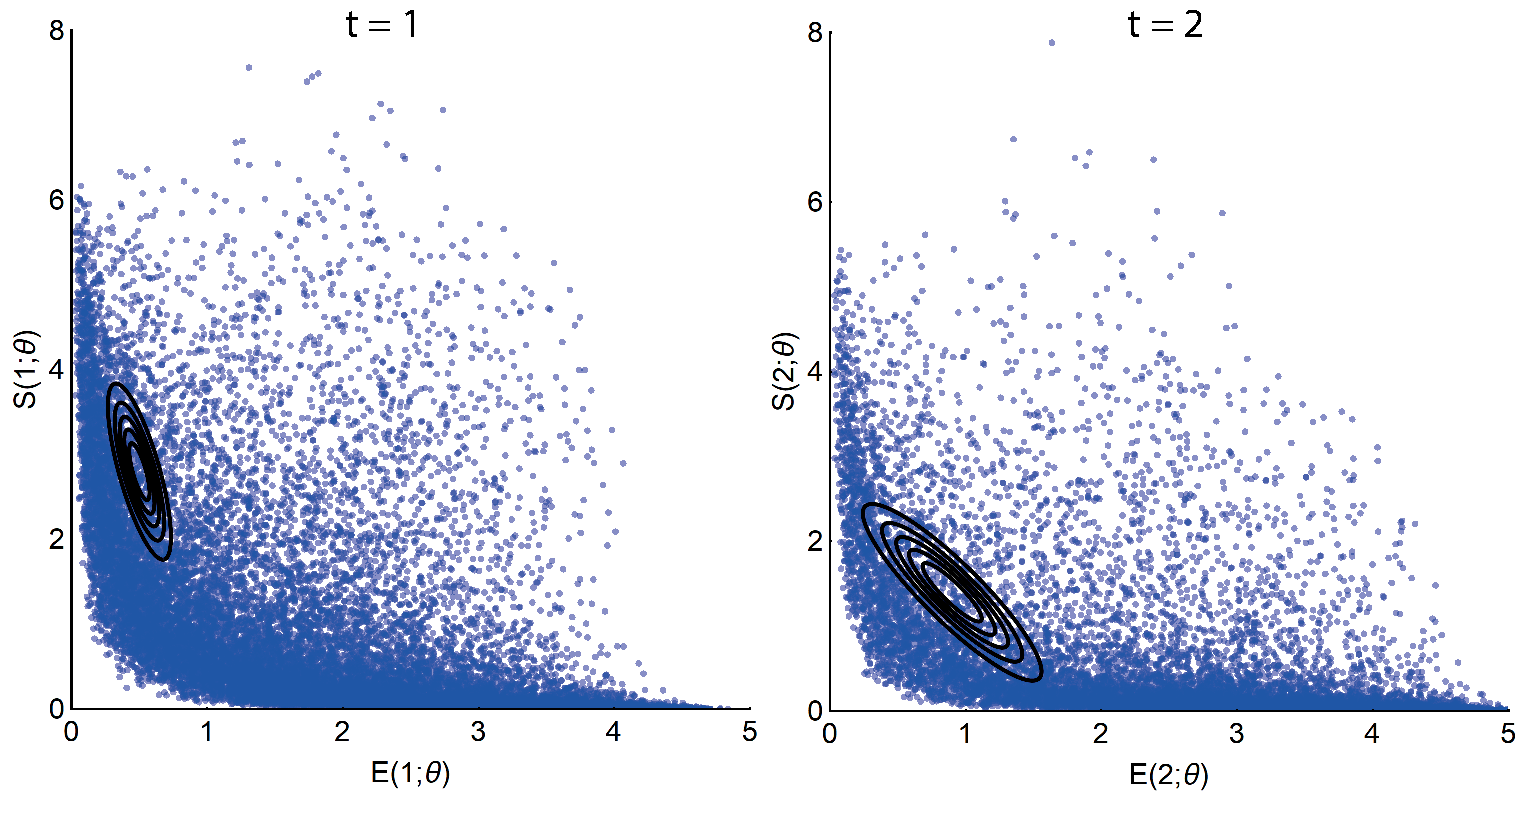
\includegraphics[width=\textwidth]{../figures/mm_4d_main.pdf}}
  \caption{\textbf{Michaelis-Menten model. QOIs (blue points) obtained by independently sampling the priors versus the target distribution (black solid contours). Left: $(q_1,q_2)$. Right: $(q_3,q_4)$.} We show 20,000 output samples, where each set of four measurements was obtained from a single sample of all parameters. The output target distribution shown by the contours corresponds to the marginal densities of each pair of enzyme-substrate measurements given by eq. (\ref{eq:MM_4d_output}).}
  \label{fig:mm_4d_main}
\end{figure}

Figure \ref{fig:mm_4d_outputs} plots the output samples of enzyme and substrate from the last step of CMC for $t=1$ (blue points) and $t=2$ (orange points) versus the contours (black lines) of the joint marginal distributions of eq. (\ref{eq:MM_4d_output}). The distribution of paired enzyme-substrate samples illustrates that the CMC output distribution closely approximates the target density, itself representing dynamic evolution of the covariance between enzyme and substrate measurements. Target marginal distributions (solid lines) along with their approximations from kernel density estimation (dashed lines) are also shown above and to the right of the main panel of Figure \ref{fig:mm_4d_outputs} and largely indicate correspondence.

\begin{figure}[H]
  \centerline{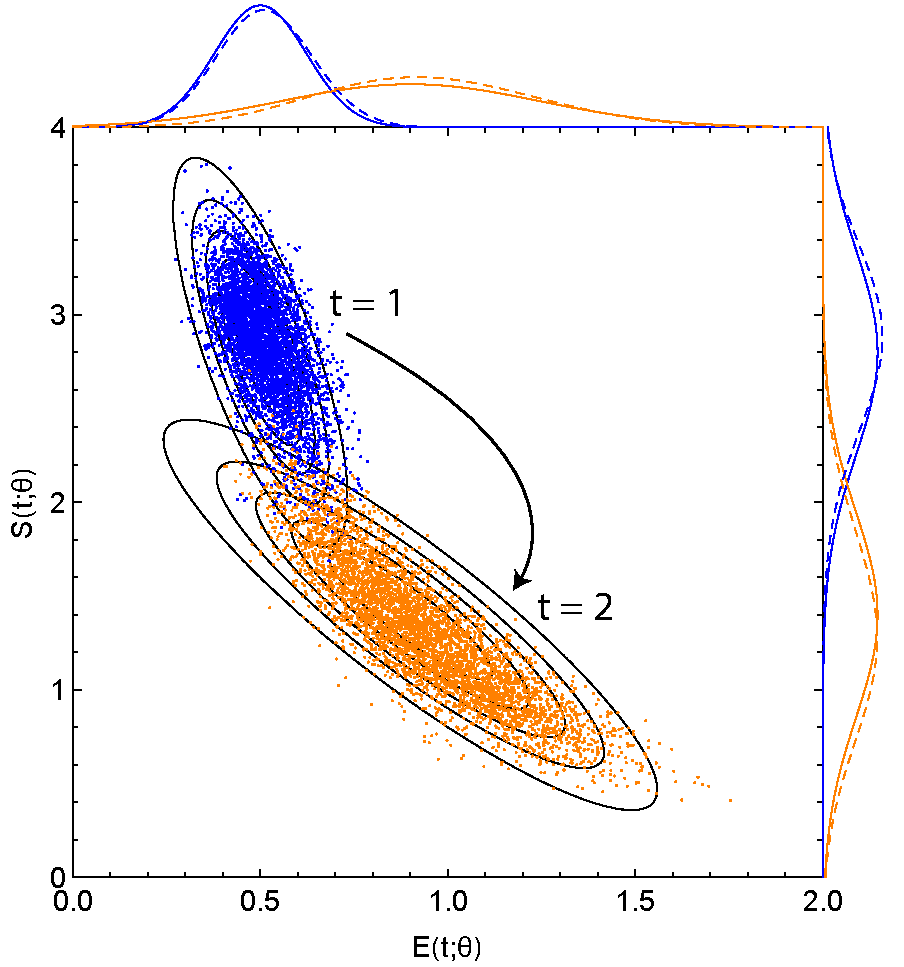
\includegraphics[width=0.65\textwidth]{../figures/mm_4d_outputs.pdf}}
  \caption{\textbf{Michaelis-Menten model. Posterior output samples from CMC (coloured points) versus contour plots (black solid lines) of the joint marginal distributions of eq. (\ref{eq:MM_4d_output}).} Enzyme and substrate measurements are given by the horizontal and vertical axes, respectively. Output functionals for $(q_1,q_2)$ and $(q_3,q_4)$ are given by blue and orange points, respectively. The solid and dashed coloured lines outside the panels indicate exact target marginals of eq. (\ref{eq:MM_4d_output}) and those estimated by CMC, respectively. In the ``ContourVolumeEstimator'' step, 200,000 independent samples were used, and in the MCMC step, 10,000 samples across each of 4 Markov chains were used, with the first half of the chains discarded as ``warm-up'' \cite{lambert2018Student}. Mathematica's ``SmoothKernelDistribution'' function, using Gaussian kernels \cite{mathematica} and bandwidths ranging from 0.1 to 0.4, was used to reconstruct marginal densities.}
  \label{fig:mm_4d_outputs}
\end{figure}


\subsection{TNF signalling pathway}
We now illustrate how CMC can be applied to another ODE system: the tumour necrosis factor (TNF) signalling pathway model introduced in \cite{chaves2008bistable} and used by \cite{hasenauer2011identification} to illustrate a Bayesian approach to cell population variability estimation. The model incorporates known activating and inhibitory interactions between four key species within the TNF pathway: active caspase 8, $x_1$, active caspase 3, $x_2$, a nuclear transcription factor, $x_3$ and its inhibitor, $x_4$, such that
%
\begin{equation}\label{eq:tnf}
\begin{aligned}
\frac{dx_1}{dt} &= -x_1(t) + \frac{1}{2}\left[\beta_4(x_3(t))\alpha_1(u(t)) + \alpha_3(x_2(t))\right]\\
\frac{dx_2}{dt} &= -x_2(t) + \alpha_2(x_1(t)) \beta_3(x_3(t))\\
\frac{dx_3}{dt} &= -x_3(t) + \beta_2(x_2(t)) \beta_5(x_4(t))\\
\frac{dx_4}{dt} &= -x_4(t) + \frac{1}{2}\left[\beta_1(u(t)) + \alpha_4(x_3(t))\right],
\end{aligned}
\end{equation}
%
with initial conditions,
\begin{equation}
x_1(0)=0.0, \quad x_2(0)=0.0, \quad x_3(0)=0.29, \quad x_4(0)=0.625.
\end{equation}
%which correspond to the steady state of the system when $x_2=0$.
The functions $\alpha_i$ and $\beta_j$ represent activating and inhibitory interactions respectively,
%
\begin{equation}
\begin{aligned}
\alpha_i(z) &= \frac{z^2}{a_i^2 + z^2}, \quad i=1, \dots, 4,\\
\beta_j(z)  &= \frac{b_j^2}{b_j^2 + z^2}, \quad j = 1, \dots, 5,
\end{aligned}
\end{equation}
%
and the parameters $a_i$ for $i\in(1,2,3,4)$ and $b_j$ for $j\in(1,2,3,4,5)$ represent activation and inhibition thresholds. The function $u(t)$ represents a TNF stimulus represented by a top hat function,
%
\begin{equation}
u(t)=\begin{cases}
1, & \text{if $t\in[0,2]$}.\\
0, & \text{otherwise}.
\end{cases}
\end{equation}
%

\subsubsection{Recovering parameter values in under-determined systems}
In under-determined models, a set of parameters of non-zero volume can produce the same output values. A consequence of this unidentifiability is that we cannot perform ``full circle'' inference: that is, using a known parameter distribution to generate an output distribution does not result in that parameter distribution being recovered through inference. We illustrate this idea by generating an output distribution by varying a single parameter value between runs of the forward model \eqref{eq:tnf} and performing inference on all nine system parameters, whilst collecting only two output measurements. Specifically, we randomly sample $a_1\sim \mathcal{N}(0.6, 0.05)$ for each simulation of the forward model, whilst holding the other parameters constant, $$(a_2,a_3,a_4,b_1,b_2,b_3,b_4,b_5)=(0.2, 0.2, 0.5, 0.4, 0.7, 0.3, 0.5, 0.4),$$ and measure $q_1=x_1(2.0)$ and $q_2=x_2(1.0)$ in each case. In doing so, we obtain an output distribution well-approximated by the bivariate Gaussian distribution,
%
\begin{equation}\label{eq:tnf_circular_target}
\begin{aligned}
\boldsymbol{q} = \begin{pmatrix} q_1 \\ q_2 \end{pmatrix}
&=
\begin{pmatrix}
x_1(2.0)\\
x_2(1.0)\\
\end{pmatrix} \\
&\sim  \mathcal{N}
\begin{bmatrix}
\begin{pmatrix}
0.26\\
0.07\\
\end{pmatrix}, \;\;
\begin{pmatrix}
2.1\times 10^{-4} & 5.9\times 10^{-5}\\
5.9\times 10^{-5} & 1.8\times 10^{-5}\\
\end{pmatrix}
\end{bmatrix}.
\end{aligned}
\end{equation}
%
We now apply CMC to the target output distribution given by eq. (\ref{eq:tnf_circular_target}) to estimate a posterior distribution over all nine parameters of eq. (\ref{eq:tnf}). Apart from a few cases, the priors for each parameter were chosen to \emph{exclude} the values that were used to generate the output distribution (see Table \ref{tab:priors}), to illustrate how the recovered posterior distribution and data generating distribution differ. In Figure \ref{fig:tnf_circular_versus}A, we plot the actual parameter values (horizontal axis) used to generate the data versus the estimated values (vertical axis). This illustrates that, due to the chosen priors, there is a disjunction between actual and estimated parameter values in all cases apart from $a_1$. Though because the model is under-determined, the corresponding output distribution closely approximates the target despite these differences (Figure \ref{fig:tnf_circular_versus}B).


\begin{figure}[H]
\centerline{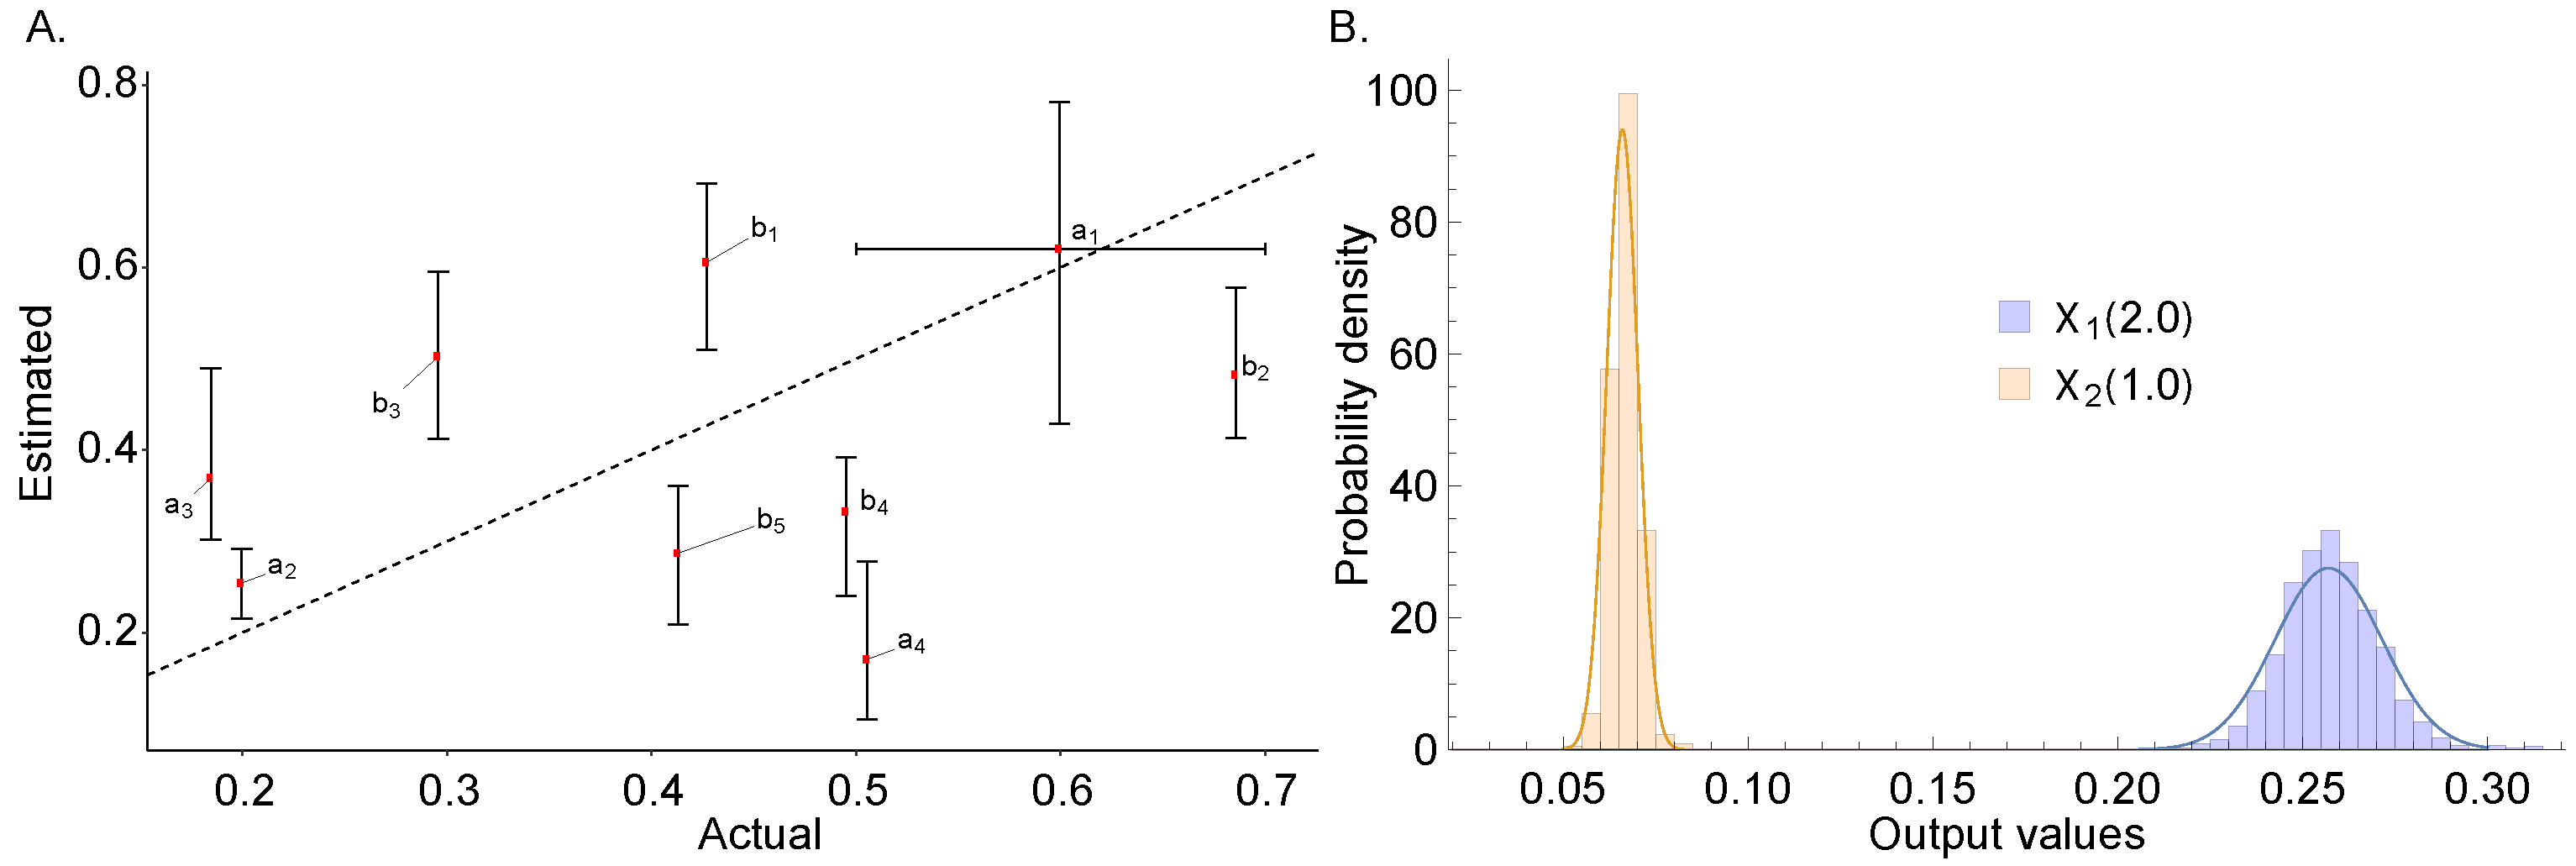
\includegraphics[width=1.0\textwidth]{../figures/tnf_circular_both.pdf}}
\caption{\textbf{TNF signalling pathway model. (A) Actual parameter values versus estimated quantiles for the output distribution of eq. (\ref{eq:tnf_circular_target}). (B) Marginal output targets (solid lines) and sampled output distributions (dashed lines).} In A, in the vertical direction, red points indicate 50\% posterior quantiles and upper and lower whiskers indicate 97.5\% and 2.5\% quantiles, respectively; in the horizontal direction, with the exception of $a_1$, red points indicate the parameter values used to generate the data; for $a_1$, the red point indicates the mean of the Gaussian distribution used to generate the data and the whiskers indicate its 95\% quantiles. In CMC, 10,000 independent samples were used in the ``ContourVolumeEstimator'' step, and 5,000 MCMC samples across each of 4 Markov chains were used in the second, with the first half of the chains discarded as ``warm-up'' \cite{lambert2018Student}. Mathematica's ``SmoothKernelDistribution'' function, using a Gaussian kernel \cite{mathematica} and a bandwidth of 0.003 was used to reconstruct marginal densities.}
	\label{fig:tnf_circular_versus}
\end{figure}

\subsubsection{Bimodal output distribution}

The dynamics of all cells can often be modelled by assuming cells exist in subpopulation clusters, which evolve differently over time. A hint that such subpopulation structure may exist is output distributions with multiple modes. We now apply CMC to investigate a bimodal output distribution for the TNF signalling pathway model similar to that investigated by \cite{hasenauer2011identification}. We aim to estimate the posterior parameter distribution mapping to the following output distribution,
%
\begin{equation}
\boldsymbol{q} = \begin{pmatrix} q_1 \\ q_2 \\ q_3 \end{pmatrix},
\end{equation}
where,
\begin{equation}
\begin{aligned}
q_1 = \boldsymbol{x}_2(1.0) &\sim \mathcal{N}(0.06, 0.01)\\
q_2 = \boldsymbol{x}_2(2.0) &\sim\frac{1}{2}\left(\mathcal{N}(0.1, 0.01) + \mathcal{N}(0.14, 0.01)\right)\\
q_3 = \boldsymbol{x}_2(4.0) &\sim\frac{1}{2}\left(\mathcal{N}(0.1, 0.01) + \mathcal{N}(0.20, 0.01)\right),\\
\end{aligned}
\end{equation}
%
where the target distributions for $\boldsymbol{q}_2(2.0)$ and $\boldsymbol{q}_2(4.0)$ indicate mixtures of univariate Gaussians, and the priors used are given in Table \ref{tab:priors}. This target distribution, along with the unique trajectories obtained by applying the CMC algorithm, are shown in Figure \ref{fig:tnf_samples_vs_distribution}. This figure illustrates that a bimodal output distribution causes CMC to sample clusters of parameter values, without the need for subpopulation information to be provided ahead of estimation.

\begin{figure}[H]
	\centerline{\includegraphics[width=0.8\textwidth]{../figures/tnf_samples_vs_distribution.pdf}}
	\caption{\textbf{TNF signalling pathway model. Target output distribution (dashed plots with grey filling) and unique trajectories (black solid lines) obtained from the posterior parameter distribution.} In CMC, 10,000 independent samples were used in the ``ContourVolumeEstimator'' step, and 5,000 MCMC samples across each of 4 Markov chains were used in the second, with the first half of the chains discarded as ``warm-up'' \cite{lambert2018Student}.}
	\label{fig:tnf_samples_vs_distribution}
\end{figure}

\begin{table}[H]
\centering
%\scriptsize
\begin{adjustwidth}{0in}{0in}%
\begin{tabularx}{1.0\textwidth}{llclcc}
Model	& Target  & Parameter & Prior    & Prior  & Prior  \\
        & density &           & density  & $\theta_1$  & $\theta_2$  \\
\toprule
Growth  & 2D     & $R_T$       & uniform & $2.5 \times 10^5$ &  $8 \times 10^5$\\
factor  & Gaussian & $k_1$       & uniform & 0.25 & 3.0\\
                && $k_{-1}$    & uniform & 2.0 & 20.0\\
                && $k_{deg}$   & uniform & 0.005 & 0.03\\
                && $k^*_{deg}$ & uniform & 0.1 & 0.5\\
\toprule
Growth  & 2D     & $R_T$ & Gaussian & $5 \times 10^5$ &  $1 \times 10^5$\\
factor  & Gaussian & $k_1$ & Gaussian & 0.5 & 0.1\\
                && $k_{-1}$ & Gaussian & 3.0 & 1.0\\
                && $k_{deg}$ & Gaussian & 0.02 & 0.005\\
                && $k^*_{deg}$ & Gaussian & 0.3 & 0.1\\
\toprule
Michaelis- & bimodal  & $k_f$ & uniform & 0.2 &  15\\
Menten     & Gaussian   & $k_r$ & uniform & 0.2 & 2.0\\
&& $k_{cat}$ & uniform & 0.5 & 3.0\\
\toprule
Michaelis- & 4D    & $k_f$ & uniform & 0.2 &  15\\
Menten     & Gaussian& $k_r$ & uniform & 0.2 & 2.0\\
&& $k_{cat}$ & uniform & 0.2 & 3.0\\
&& $E_0$ & uniform & 3.0 & 5.0\\
&& $S_0$ & uniform & 5.0 & 10.0\\
&& $C_0$ & uniform & 0.0 & 0.2\\
&& $P_0$ & uniform & 0.0 & 0.2\\
\toprule
TNF & bivariate & $a_1$ & uniform & 0.4 & 0.8\\
signalling & Gaussian& $a_2$ & uniform & 0.1 & 0.7\\
&& $a_3$ & uniform & 0.3 & 0.7\\
&& $a_4$ & uniform & 0.1 & 0.3\\
&& $b_1$ & uniform & 0.5 & 0.7\\
&& $b_2$ & uniform & 0.4 & 0.6\\
&& $b_3$ & uniform & 0.4 & 0.6\\
&& $b_4$ & uniform & 0.2 & 0.4\\
&& $b_5$ & uniform & 0.2 & 0.4\\
\toprule
TNF  & bimodal  & $a_1$ & uniform & 0.5 & 0.7\\
signalling& Gaussian & $a_2$ & uniform & 0.1 & 0.3\\
&& $a_3$ & uniform & 0.1 & 0.3\\
&& $a_4$ & uniform & 0.4 & 0.6\\
&& $b_1$ & uniform & 0.3 & 0.5\\
&& $b_2$ & uniform & 0.6 & 0.8\\
&& $b_3$ & uniform & 0.2 & 0.4\\
&& $b_4$ & uniform & 0.4 & 0.6\\
&& $b_5$ & uniform & 0.3 & 0.5\\
\toprule
hESC & 1D-2D & $p_1$ & uniform & 40.0 & 60.0\\
differentiation & Gaussian & $p_2$ & uniform & 2.0 & 10.0\\
&& $p_3$ & uniform & 0.5 & 16\\
&& $p_4$ & uniform & 0.0 & 0.7\\
&& $p_5$ & uniform & 2.0 & 4.0\\
&& $p_6$ & uniform & 2.0 & 20.0\\
&& $p_7$ & uniform & 0.0 & 0.2\\
\end{tabularx}
\caption{\textbf{Priors used for each example in \S\ref{sec:results}.} The parameters $\theta_1$ and $\theta_2$ indicate the prior hyperparameters: for uniform priors, these correspond to the lower and upper limits; for Gaussian priors, they correspond to the mean and standard deviation.}
\label{tab:priors}
\end{adjustwidth}
\end{table}

\subsection{Embryonic stem cell differentiation}\label{sec:hesc}
We now demonstrate how CMC can be applied to real data generated from experiments investigating human embryonic stem cell (hESC) differentiation. Specifically, we use a reaction kinetics-based model derived from the ODE system presented in \cite{tu2019single}, which seeks to explain regulation of three transcription factors involved in hESC fate: CDH1, ZEB1 and KLF8. This system was modelled by the following system, involving a number of Michaelis-Menten-type terms,
%
\begin{equation}
\begin{aligned}
\frac{d C}{d t} &= \frac{k_1}{k_2 + Z^2} + \frac{k_3}{k_4 + K^2} - d_1 C\\
\frac{d Z}{d t} &= \frac{a k_5 K^2}{k_6 + K^2} - d_2 Z\\
\frac{d K}{d t} &= \frac{r k_7}{k_8 + C^2} - d_3 K,
\end{aligned}
\end{equation}
%
where $C=[\text{CDH1}]$, $Z=[\text{ZEB1}]$ and $K=[\text{KLF8}]$, subject to initial conditions: $C(0) = C_0, Z(0)=Z_0, K(0) = K_0$, and $a=1$ and $r=1$ are nondimensional parameters. We recast this system, using the following nondimensional variables (see supplementary files for further details):
%
\begin{equation}
y_1 = \frac{k_2 d_1}{k_1} C, \; y_2 = \frac{k_6 d_1}{k_4 k_5} Z, \; y_3 = \frac{1}{\sqrt{k_4}} K,
\end{equation}
%
and time scale $\frac{1}{d_1}$, so that $\tau = d_1 t$, which results in the following system,
%
\begin{equation}\label{eq:tu_nondimensional}
\begin{aligned}
\frac{d y_1}{ d\tau} &= \frac{1}{1 + p_1 y_2^2} + \frac{p_2}{1 + y_3^2} - y_1\\
\frac{d y_2}{ d\tau} &= \frac{y_3^2}{1 + p_3 y_3^2} - p_4 y_2\\
\frac{d y_3}{d\tau} &= \frac{p_5}{p_6 + y_1^2} - p_7 y_3,
\end{aligned}
\end{equation}
%
with initial states $y_1(0) = y_{1,0}, y_2(0) = y_{2,0}, y_3(0) = y_{3,0}$.

In what follows, we perform parameter inference for eq. \eqref{eq:tu_nondimensional} on single-cell RNA-seq data obtained and processed as described in \cite{tu2019single} from NCBI's Gene Expression Omnibus. The dataset has single-cell gene expression data for 758 cells collected at six times during the course of experiment (0 h, 12 h, 24 h, 36 h, 72h, 96 h) for [CDH1], [ZEB1] and [KLF8] with 92, 102, 66, 172, 138 and 188 measurements at each time point respectively.


Here, we consider estimating the posterior parameter distributions using data obtained at $t=12 \text{h}$ for CDH1 and $t=72 \text{h}$ for KLF8. Across the three cases described below, we use CMC with priors for parameters in eq. \eqref{eq:tu_nondimensional} as given in Table \ref{tab:priors}. We assume the initial values of each variable are given by: $y_1(0) = 1.5, y_2(0) = 0.0, y_3(0) = 0.0$.

We first consider the CDH1 data in isolation: to do so, we fit a Gaussian distribution to these data and obtain $q_1=y_1(12)  \sim \mathcal{N}(5.50, 1.05)$. CMC produces samples that closely approximate this distribution (Figure \ref{fig:tu_outputs}A; blue lines). The joint posterior distribution for two model parameters, $(p_2, p_5)$, is shown in the leftmost panel of Figure \ref{fig:tu_inputs} and shows a concentrated distribution.

Next we consider the KLF8 data: we fit a Gaussian distribution to these and obtain $q_2=y_3(72)  \sim \mathcal{N}(3.77, 1.37)$.  Again, using CMC, we obtain samples that closely approximates this target (Figure \ref{fig:tu_outputs}A; orange lines). The posterior distribution for $(p_2, p_5)$ is, however, now quite different to previously (Figure \ref{fig:tu_inputs} middle panel) hinting that it may be quite difficult to determine a posterior distribution where we target both $q_1$ and $q_2$.

Finally, we attempt to target the distribution described by both $q_1$ and $q_2$: here, we assume that there is no correlation between these targets because we have no cells with observations for both $t=12$ and $t=72$ since the measurement process is destructive. In Figure \ref{fig:tu_outputs}B, we plot the joint target distribution and samples from CMC. In this plot, it is clear that there is a disjunction between the target distribution and the samples. In particular, the target distribution for $q_2$ has a mean that is far below the target value.

The rightmost panel of Figure \ref{fig:tu_inputs} shows the posterior parameter distribution for $(p_2, p_5)$ when targeting this bivariate output distribution. In comparing it to the other panels in the same figure, it is clear that the posterior distribution when targeting $(q_1,q_2)$ is somewhere between the distributions obtained when targeting $q_1$ and $q_2$ in isolation; unfortunately, this midway house is not suited to either case, however. Indeed, this failure to target both $q_1$ and $q_2$ simultaneously suggests that the model does not actually cohere with the data.

\begin{figure}[H]
	\centerline{\includegraphics[width=1\textwidth]{../figures/tu_outputs.png}}
	\caption{\textbf{Embryonic stem cell differentiation model: output targets.} In A., we show the output target distributions described in \S\ref{sec:hesc} and kernel density estimates of the distributions reconstructed from the CMC samples. In B., we show the joint target distribution (contour lines) for the case where we target both $q_1$ and $q_2$ simultaneously; above and to the right of the plot, we show the target marginals (solid lines) and the marginals reconstructed from the samples (dashed lines). In CMC, 50,000 independent samples were used in the ``ContourVolumeEstimator'' step, and 50,000 MCMC samples across each of 4 Markov chains were used in the second, with the first half of the chains discarded as ``warm-up'' \cite{lambert2018Student}. Mathematica's ``SmoothKernelDistribution'' function, using a Gaussian kernel \cite{mathematica} and default bandwidths were used to reconstruct marginal densities.}
	\label{fig:tu_outputs}
\end{figure}

\begin{figure}[H]
	\centerline{\includegraphics[width=1\textwidth]{../figures/tu_inputs.png}}
	\caption{\textbf{Embryonic stem cell differentiation model: posterior parameter distribution.} In the left panel, we show the posterior distribution for $(p_2, p_5)$ when targeting $q_1$; in the middle, we show the same when targeting $q_2$; and in the right panel, we show the same when targeting $(q_1, q_2)$. In CMC, 50,000 independent samples were used in the ``ContourVolumeEstimator'' step, and 50,000 MCMC samples across each of 4 Markov chains were used in the second, with the first half of the chains discarded as ``warm-up'' \cite{lambert2018Student}.}
	\label{fig:tu_inputs}
\end{figure}

To investigate this further, we overlay samples (blue points) from the contour volume estimation step of Algorithm \ref{alg:cmc} on the joint target distribution of $(q_1,q_2)$ in Fig. \ref{fig:tu_contours}. In the main panel, the output samples are concentrated in a band that runs from the top left of the plot towards the lower right. Because of this, there is relatively low overlap between the joint target and the contour volumes, indicating that the model does not cohere well with the data and illustrates why inference struggles to find a posterior distribution consistent with the joint target. However, as illustrated in Fig. \ref{fig:tu_outputs}A, it is possible to find posterior distributions consistent with the target distributions for either $q_1$ or $q_2$ in isolation. Fig. \ref{fig:tu_contours} indicates why this is the case: above the main panel, we plot these target distributions (black solid lines) and the corresponding contour volume distributions (blue dashed lines). There is considerably more overlap in these marginals than in the joint densities, which shows that finding a posterior consistent with each of these targets in isolation is possible but with them both is tricky. Overall, it appears that the model is not consistent with the data.

\begin{figure}[H]
	\centerline{\includegraphics[width=0.7\textwidth]{../figures/tu_contours.png}}
	\caption{\textbf{Embryonic stem cell differentiation model: contour volume distribution.} In the main panel, we plot contours (solid black lines) for the joint target distribution of $(q_1,q_2)$ and 20,000 samples from the contour volume estimation step of Algorithm \ref{alg:cmc} (blue points). Above and to the right of the main panel, we plot the marginal target distribution in each dimension (solid black lines) and the marginal contour volume distributions (dashed blue lines).}
	\label{fig:tu_contours}
\end{figure}

 By ``model'' here, it could either be that the ODE system described in eq. \eqref{eq:tu_nondimensional} is inappropriate; it is also possible that this could be due to failure to include noise in the measurement process. Given the extent of the discrepancy between the ODE means and the target contours, we suggest that it's most likely that the ODE model misses or misrepresents key processes. These results illustrate how CMC can be used to determine when a model is inconsistent with data and also suggest that extending CMC to handle noisy measurement is likely worthwhile.



\section{Discussion}
\label{sec:discussion}
Determining the cause of variability in cellular processes is crucial in many applications, ranging from bioengineering to drug development. In this paper, we introduce a Bayesian method for estimating cellular heterogeneity from ``snapshot'' measurements of cellular properties, taken at discrete intervals during experiments. Our approach assumes what we call a ``heterogeneous ordinary differential equation'' (HODE) framework, in which biochemical processes in all cells are governed by a common ODE. In HODEs, each cell has different rate parameter values, causing a variety of measurements to be obtained across cells. In this framework, estimating heterogeneity in cellular processes amounts to determining the probability distributions of parameter values of the governing ODE. Our method of estimation is a two-step Monte Carlo sampling process we term ``Contour Monte Carlo'' (CMC), which does not require the number of cell clusters to be provided before estimation, unlike in other approaches. CMC can be used to process high volumes of individual cellular measurements since the framework involves fitting a kernel density estimator to raw experimental data and using these distributions rather than data as the target outcome. CMC can handle arbitrary multivariate structure in measured outputs, meaning it can capture correlations between the same cellular species at different timepoints or, for example, contemporaneous correlations between different cellular compartments. Being a Bayesian approach, CMC uses prior distributions over parameter values to ensure uniqueness of the posterior distribution, allowing pre-experimental knowledge to be used to improve estimation robustness. The flexible and robust framework that CMC provides means it can be used to perform automatic inference for wide-ranging systems of practical interest.

Our approach also provides a natural way to test that the process is working satisfactorily. Feeding posterior parameter samples obtained by CMC into forward model simulations results in a distribution of output values which can be compared to the target. Indeed, we have found this comparison indispensable in applying CMC in practice and include it as the last step in the CMC algorithm (Algorithm \ref{alg:cmc}). Discrepancies between the target output distribution and its CMC approximation can occur either as a result of poor estimates of the ``contour volume distribution'' in the first stage of the algorithm or due to insufficient MCMC samples in the second. Either of these issues are often easily addressed by increasing sample sizes or changing hyperparameter settings for the kernel density estimator. Although kernel density estimation in high dimensional spaces remains an open research problem, we have found vine copula kernel density estimation works well for the dimensionality of output measurements we investigate here \cite{nagler2016evading}.

Failure to reproduce a given output distribution can also indicate that the generating model (the priors and the forward model) are incongruent with experimental results. This may either be due to misspecification of the ODE system or because the assumption of a deterministic forward model is inappropriate. Our approach currently assumes that output variation is dominated by cellular variation in the parameter values of the underlying ODE, with measurement noise making a negligible contribution. Whether this is a reasonable assumption depends on the system under investigation and, more importantly, on experimental details. We recognise that neglecting measurement noise when it is, in fact, important in determining observed data means CMC will overstate cellular variation. It may also mean that some output distributions cannot be obtained by our model system (i.e. HODEs without noise). Future work incorporating a stochastic noise process or, more generally, including stochastic cellular mechanisms is thus likely to be worthwhile.

In Figure \ref{fig:workflow}, we present the workflow for our approach, which includes as its last step comparing output samples with the target distribution. As discussed above, if output samples do not correspond with the target, this may indicate that a model isn't fit for purpose. Conversely, if there is correspondence with the target distribution, it is possible that a simplified model -- with (say) one or more fewer parameters -- could also recapitulate the same results. Thus, a process of repeated rounds of model simplification then CMC could be pursued to simplify a model until output samples no longer correspond with the target. The most parsimonious model would then be the simplest case where the output samples still match the target. We note however, that such an approach may be dangerous if the most parsimonious model is then used to predict the distributions of other functionals.

Whilst we have illustrated our approach by fitting ODE models to data, we recognise that our approach is applicable to deterministic forward models in general. These include a large swathe of models used in computational biology, such as partial differential equations and difference equations. Similarly, whilst we have illustrated our approach by fitting to models with time-invariant parameters, it could also be used to determine how parameters vary throughout the course of an experiment - provided the dynamic evolution of parameter values is itself parameterised.

We have labelled our approach as Bayesian since it involves explicit estimation of probability distributions and requires priors. We recognise, however, that it is not of the form used in traditional Bayesian inference. This is because, rather than aiming to formulate a model that describes output observations, our approach aims to recapitulate output \emph{distributions}. Others \cite{BJW-18}, (including us \cite{lambert2018inverse}), have considered similar problems before; perhaps most notably by Albert Tarantola in his landmark work on inverse problem theory (see, for example, \cite{tarantola2005inverse}). In Tarantola's framework, a joint input parameter and output space is considered, where prior knowledge and experimental theory combine elegantly to produce a posterior distribution whose marginal output distribution is a weighted ``conjunction'' of various sources of information. This work has seen considerable interest in areas such as the geosciences \cite{mosegaard1995monte,vukicevic2008analysis}, and we propose that Tarantola's approach may prove useful for the biosciences.


The natural world is rife with variation, and mathematical models represent frameworks for understanding its causes. Typically, the state of biological knowledge is such that one effect -- a given pattern of variation -- has many possible causes. Observational or experimental data can be used to apportion weight to each cause, in a process that amounts to solving an inverse problem. The approach we describe here follows the Bayesian paradigm of inverse problem solving where uncertainty in potential causes (i.e. parameter values) is described using probability distributions. Here, we illustrate the worth of our method by using it to estimate cellular heterogeneity in biochemical processes. However, it could equally be used to invert other classes of under-determined systems arising elsewhere. Contour Monte Carlo provides an automatic framework for performing inference on such under-determined systems, and the use of priors allows for robust and precise parameter estimation unattainable through the data alone.




\section{Author contributions}
BL, DJG and SJT conceived the study. BL carried out the analysis. All authors helped to write and edit the manuscript.


\nolinenumbers

\bibliographystyle{unsrt}
\bibliography{Bayes}
\end{document}

